\documentclass[12pt]{report}
\usepackage[mathletters]{ucs}
\usepackage[utf8x]{inputenc}
\usepackage{hyperref}
\usepackage[english,spanish]{babel}
\usepackage{amsmath}
\usepackage{amssymb}
\usepackage{usmtesis/usmtesis}
\usepackage[noBBpl]{mathpazo}
\usepackage[small,labelfont=bf]{caption}
\usepackage{subfigure}
\usepackage{tikz}
\usepackage{listings}
\usepackage[textsize=tiny]{todonotes}
\usepackage{booktabs}
\usepackage{graphicx}
\usepackage{tabularx}
\usetikzlibrary{calc,arrows,patterns,decorations,snakes}

\lstset{basicstyle=\ttfamily\footnotesize,backgroundcolor=\color{gray!10}}

\hyphenation{Fede-rico}

\ingciv
%\nolistoftables
\nolistoffigures
\copyrightyear{2013}
\submitdate{Diciembre 2013}
\convocation{Diciembre}{2013}

\title{%
  Modelo de calidad
  para evaluar
  continuidad de desarrollo
  }
\author{Pablo Alejandro Acuña Rozas}

\begin{document}
\profguia{Dr.~Hernán Astudillo}
\profcorr{Dr.~Raúl Monge}

\beforepreface
\afterpreface
\selectlanguage{spanish}
\chapter{Introducción}
En este trabajo se propone un modelo de calidad para evaluar la continuidad
de desarrollo de un producto de software, así como las tareas necesarias
para llevar a cabo una evaluación de calidad.
La base de este modelo se encuentra en la serie ISO 25000
específicamente en la subdivisión de modelo de calidad.
Se han realizado ajustes para adaptar y refinar el modelo con el fin de evaluar la mantenibilidad de un producto de software.
Esta característica influye directamente en la continuidad de desarrollo y puede
ser descrita a través subcaracterísticas y métricas que sean capaz de cuantificarlas.

Se presenta también una aplicación del modelo generado, sobre un producto de software
real, con el fin de mostrar los pasos principales a la hora de llevar a cabo
una evaluación de calidad y para ejemplificar el uso del framework propuesto. Este framework se compone
del modelo de mantenibilidad y del proceso para llevar a cabo la evaluación.

En el capítulo~\ref{chap:contexto} se introducen los principales conceptos trabajados
en esta memoria y el contexto sobre el cuan han sido abordados.

El problema principal es presentado en el capítulo~\ref{chap:problema} así como
los problemas secundarios que se ramifican de este. El estado del arte relacionado
con el problema se puede encontrar en el capítulo~\ref{chap:arte}

La propuesta de modelo de mantenibilidad así como la descripción de las tareas del proceso
de evaluación son descritos en el capítulo~\ref{chap:propuesta}. En esta sección
también se mencionan las principales características del modelo base del cual
se refinó el modelo de mantenibilidad.

La validación del modelo se puede encontrar en el capítulo~\ref{chap:validacion}.
Para esta sección se realizó una evaluación de calidad sobre un producto de software
real. Se describen las tareas del proceso de evaluación, así como los resultados
de la aplicación del modelo generado con el fín de certificar que el software
cumple con el criterio de evaluación definido.

Finalmente las conclusiones del trabajo son descritas en el capítulo~\ref{chap:conclusiones}.

%hablar sobre calidad, mantenibilidad y su principal función en el desarrollo.

\chapter{Contexto}

%sobre calidad
\section{Calidad de Software}
Calidad de Software es un tema tremendamente importante en el proceso de desarrollo.
Hoy en día sabemos que un producto de software que no cuenta con los estándares de
calidad adecuados, no goza de propiedades como mantenibilidad, seguridad, usabilidad, etc.
Si bien la calidad en general es un concepto subjetivo, se han desarrollado un gran
número de intentos por definir una base común con la cual se pueda evaluar un producto 
de software o que sirva para definir un desarrollo apropiado con el fin de terminar
con un producto confiable. Estos intentos generalmente apuntan a definir un modelo
de calidad que agrupe las principales características que un producto debe tener.

La ISO, IEC y IEEE definen calidad a través de 6 distintas alternativas~\cite{5276043}:
\begin{enumerate}
    \item El grado en el cual un sistema, componente o proceso cumple con los requerimientos especificados.
    \item La calidad de un producto, servicio, sistema o proceso para cumplir con las necesidades, expectativas
    o requerimientos del usuario o cliente.
    \item El conjunto de características de una entidad que le confieren su habilidad de satisfacer los requerimientos
    declarados y además los implícitos.
    \item Conformidad en las expectativas del usuario, conformidad en los requerimientos del usuario, satisfacción del cliente,
    confiabilidad y el nivel presente de defectos.
    \item El grado en el cual un conjunto inherente de características cumple con los requerimientos.
    \item El grado en el cual un sistema, componente o proceso cumple con las necesidades o expectativas de un ciente o usuario.
\end{enumerate}

Como se puede observar en las definiciones, calidad no tiene una definición universal e incluso se podría argumentar
que es un tema de carácter filosófico~\footnote{\url{http://en.wikipedia.org/wiki/Quality_(philosophy)}}.

Un modelo clásico de calidad de producto, que puede ser aplicado en productos
de software es el de Garvin~\cite{Garvin:1984}. Garvin presenta los siguientes
enfoques que se pueden utilizar dentro de calidad:
\begin{itemize}
    \item Enfoque trascendente
    \item Enfoque basado en el producto
    \item Enfoque basado en el usuario
    \item Enfoque de fabricación
    \item Enfoque basado en valor
\end{itemize}

El enfoque trascendente es el más difuso. Se refiere a la propiedad inherente
e indefinible de un producto, con la cual cumple con una alta calidad. Podría
decirse que es casi una característica intuitiva con la cual se sabe si un
producto es de calidad.

El enfoque basado en producto describe diferencias en la cantidad de algunos
atributos deseados en el producto. Por lo tanto a diferencia del enfoque
trascendente, este enfoque puede ser medido. Asumimos que se conoce
y se puede describir lo que se desea.
Este enfoque es complicado en productos de software puesto que algunas métricas
pueden no existir o ser muy difíciles de medir. Un ejemplo es la mantenibilidad.
Si se asocia mantenibilidad al esfuerzo requerido para completar un cambio, este
esfuerzo es difícil de medir a través de diversos desarrolladores ya que no están
constantemente midiendo el tiempo en sus respectivas tareas. Además depende de 
otros factores como la complejidad del cambio.

En el enfoque basado en usuario, se asume que el producto que satisface
las necesidades del usuario de mejor manera, tiene la mejor calidad. El énfasis
no está en los requerimientos, sino en la impresión subjetiva de los usuarios.

Una visión más interna se observa en el enfoque de fabricación. En este enfoque
calidad se define como la conformidad con respecto a los requerimientos especificados.
Se debe asumir que siempre será posible definir un requerimiento así como la desviación
del producto real con respecto a este requerimiento. En este enfoque las métricas
concretas, por ejemplo defectos por linea de código son más útiles mientras puedan
relacionarse con algún requerimiento especificado.

Finalmente en el enfoque basado en valor se asignan costos a la conformidad y no
conformidad con respecto a requerimientos, se comparan con los beneficios del
producto y con estos datos se calcula su valor.

Garvin sugiere que estos distintos enfoques puede ser útiles durante distintas
etapas del ciclo de vida del producto. Por ejemplo, al inicio del ciclo de 
vida, durante la incepción del producto, debemos enfocarnos más en el usuario
y en el valor, con el fin de entender que es lo que tiene más valor para
los clientes y usuarios. O por ejemplo, cuando se está construyendo el producto,
debemos concentrarnos más en la fabricación, con el fin de asegurar que se está
construyendo un producto adecuado con respecto a la especificación.

\subsection{Calidad de procesos}
Otra parte importante de calidad que es fuertemente estudiada es la calidad de 
procesos. La principal idea detrás de este enfoque, es que mientras de más
calidad sean los procesos, de más calidad serán los productos.

Un estándar altamente utilizado en la calidad de procesos es la ISO 9000. La idea
consiste en establecer un sistema de gestión de calidad en una compañía de
manera que la calidad resultante del producto también sea alta. No tiene que ver
directamente con la calidad del producto, sino con los requerimientos de calidad
de la compañía que produce el producto. 
La introducción de este tipo de estándares dentro de una compañía de software
puede beneficiarla al hacer que los procesos de aseguramiento de calidad sean
más explícitos y claros~\cite{Wagner:2013}.

Otras iniciativas similares, que se enfocan específicamente en mejorar los
procesos de desarrollo de software son CMMI y SPICE.
Estos estándares se basan en la premisa de que existe un proceso ideal, 
el cual es descrito en los estándares y que cada compañía debe alcanzar.
Existen niveles de madurez y de capacidad partiendo desde procesos caóticos,
hasta procesos altamente estandarizados y optimizados.

La utilización de este enfoque para evaluar continuidad de desarrollo sufre
de ciertas carencias. Para empezar se parte con la premia de que mientras
mejores sean los procesos, mejor será la calidad del producto. Esto quizás
es claro en fabricación de productos, pero no tan claro en desarrollo de
software. Por ejemplo en~\cite{Jones:2000:SAB:335582} se presenta una 
investigación que buscaba la relación entre el nivel CMM (predecesor de CMMI) 
de una compañía, y el número de defectos por punto de función entregado en sus productos.
Como resultado se encontró que mientras el nivel aumentaba, los errores disminuían,
lo cual confirmaría la premisa. Sin embargo en los extremos, las mejores
compañías que estaban en nivel CMM 1 (el peor), producían software con menos
defectos que las peores compañías con CMM 5 (el mejor). Por lo tanto
existe otros factores que estaban influyendo en la tasa de defectos.

Es importante analizar la calidad de procesos para lograr entregar un producto
de software de alta calidad, sin embargo como muchos otros factores influyen
en la industria del software, este trabajo está más enfocado en estudiar
la calidad del producto, y a través de esta calidad encontrar un modelo que
permita evaluar también la continuidad de desarrollo.

\section{Mantenibilidad}

%sobre mantenibilidad
La mantenibilidad también es un tema recurrente en ingeniería de software.
Al igual que calidad, se compone de elementos subjetivos y que están sujetos
al contexto del problema. Para medir la mantenibilidad de un producto de
software, se suelen utilizar métricas cuantitativas y cualitativas. Estas
métricas usualmente indican que tan mantenible es el producto.
Esto puede implicar diversos hechos, por ejemplo, que tan fácil es modificar
el código fuente del software, que tan seguro es la modificación del código
fuente sin dañar el funcionamiento correcto del sistema, que tan fácil es entender el código
fuente del software con el fin de modificarlo o extenderlo, etc.
Esta característica de calidad afecta generalmente a los desarrolladores,
puesto que el usuario final no es afectado directamente por la buena calidad
del código fuente, mientras el software cumpla con los requerimientos de usuario.
Sin embargo es frecuente escuchar sobre proyectos que han debido ser paralizados
producto de falta de calidad en su código, lo cual no permite seguir
manteniéndolo.


\chapter{Problema}
\label{chap:problema}
El problema principal consiste en la falta de un modelo de calidad apropiado
que permita evaluar la continuidad de desarrollo de un producto de software.
Este modelo debe estar enfocado en los aspectos que más contribuyan a la mantenibilidad
del producto, ya que, como se mencionó previamente, esta es la característica que más
influye en la continuidad de desarrollo.
Cuando este desarrollo es tomado por terceros, la mantenibilidad
del software se torna crítica, ya que afecta directamente a todos los procesos y tareas
que este desarrollo conlleva, ya sea la mantención, eliminación de fallas, análisis de código,
extensión del software, reutilización de módulos o funciones, etc.

El problema secundario aparece una vez definido el modelo principal, con sus características
y subcaracterísticas. Para realizar una evaluación sobre un producto de software real, se deben
utilizar métricas que representen y den un valor medible a estas subcaracterísticas.
Esta elección debe ser apropiada y acorde a las prácticas y estándares utilizados en la industria
hoy en día.

Además de las métricas, se debe diseñar un proceso de evaluación que sirva como guía a los
evaluadores y que permita realizar las tareas de evaluación de manera sistemática y organizada, 
siempre tomando en cuenta el contexto del problema. 

Teniendo estos componentes: el modelo de calidad con sus características y subcaracterísticas,
la métricas que dan valor medible a estas subcaracterísticas, y las tareas correspondientes al proceso de evaluación, 
se puede llevar a cabo una evaluación exitósa sobre el producto de software.

%e.a para continuidad de desarrollo
\chapter{Estado del arte}

La continuidad de desarrollo está ligada directamente con la mantenibilidad
de un producto de software. Cuando el desarrollo del producto es tomado
por terceros, esta característica se torna más crítica.

El estudio acerca de como medir la mantenibilidad y de como crear sistemas
más mantenibibles, ya sea para agregar nuevas características o arreglar
errores, tiene varios años de estudio en la literatura de ingeniería de Software.
A continuación se presentan los principales estudios acerca de mantenibilidad
de software y de los distintos acercamientos para abordar el problema
de evaluar la mantenibilidad de un producto.

\section{Estudios acerca de Mantenibilidad de Software}

Ya en la década de los años noventa, se consideraba que la mantenibilidad
de software era un tema fundamental y que podía generar un impacto notorio
en el costo de mantenimiento de un producto de software. En \cite{Oman:1992}
se definen ciertas métricas para realizar mediciones de mantenibilidad y se
presenta un índice de mantenibilidad que permite unificar estas métricas en
una sola.

Uno de los estudios conocidos de esta época se puede encontrar en \cite{Coleman:1996}.
En este trabajo altamente citado se presentan guías  para automatizar el análisis de
mantenibilidad con el fin de apoyar la toma de decisiones relacionadas con el
software en cuestión. Se evaluaron 5 métodos utilizando datos reales y luego
se menciona como estos métodos pueden ser utilizados en un ambiente industrial.
Los modelos aplicados fueron: modelos jerárquicos multidimensionales, modelos
de regresión polinomial, medidas de complejidad basadas en entropía, análisis
de componentes principales y análisis de factores.

Otro trabajo importante llevado a cabo en esta década es
presentado en \cite{West:1996}. Se presentan algunas definiciones
relativas a mantenibilidad de software así como la importancia que tiene
este atributo en cualquier sistema. Además se presenta un método básico
para evaluar mantenibilidad utilizando dos indicadores principales: la
medida de mantenibilidad (MM) y el índice de mantenibilidad (MI). Este último
es utilizado hasta hoy en día para tener una referencia rápida del comportamiento
estático de un sistema. 

Ya para los siguientes años, el tema de mantenibilidad de software es considerado
de alta importancia y se puede encontrar diversos estudios que resumen y presentan
el estado del arte del área. A continuación se nombran los más relevantes
para esta memoria.

En \cite{survey} se presentan los principales factores que afectan a la mantenibilidad de
software. Estos factores son extraídos de diferentes autores los cuales 
proponen diferentes modelos de mantenibilidad de software.
En el desarrollo del reporte se presentan factores tales como 
analizabilidad, modificabilidad, estabilidad, capacidad de pruebas, modularidad,
descriptividad, consistencia, simplicidad, etc. Estos son tomados de modelos
conocidos tales como el modelo de calidad de la ISO 9126, el modelo de calidad
de Boehm, modelo de McCall, el modelo Fuzzy, modelo MEMOOD, etc.

En \cite{roadmap} se describen guías para estudiar la mantenibilidad de software
utilizando métricas basadas en orientación a objetos. Para este estudio
se generó un catálogo de investigaciones importantes relevantes utilizando
ciertas heurísticas. Se encontraron 606 métricas de las cuales 570 eran métricas
orientadas a objectos y 71 métricas orientadas a aspectos. Otro resultado
interesante que surgió del estudio fueron los tópicos encontrados al buscar
investigaciones relacionadas con mantenibilidad. Estos fueron limitaciones
de arquitectura de software, herencia, cohesión, acoplamiento, complejidad
y tamaño. De estos conceptos se encontró que cohesión y acoplamiento eran
los tópicos mayormente investigados en la literatura con respecto a mantenibilidad.

Otro estudio relacionado con mantenibilidad enfocada en orientación a objectos
se puede encontrar en \cite{pastDecade}. En este trabajo se revisan estudios
de métricas de mantenibilidad de software orientado a objectos correspondientes
a la década pasada (2003-2012). Del estudio se concluyó que los métodos
basados en análisis de regresión (RA) fueron los mayormente empleados para
evaluación durante la década. Otros modelos de calidad existentes tales como
ISO 9126 o el modelo de McCall son escasamente utilizados en el desarrollo
de modelos de mantenibilidad. La mayoría de los estudios obtenidos en la investigación
hacen uso de las métricas orientadas a objetos existentes sin una revisión
y adaptación crítica antes de ser utilizadas para desarrollar modelos.

Otro estudio de métricas existentes para software orientado a objectos se puede
encontrar en \cite{TowardsACatalog}. En este trabajo se discuten un rango de
opciones para categorizar métricas. Lo que se buscar es solucionar el problema
de la falta de información útil acerca de métricas para mantenibilidad de 
software orientado a objetos que apoye la toma de decisiones acerca de cuales
de estas métricas debiesen ser adoptadas en estudios académicos o incluso
en actividades del día a día en la industria del software. Este trabajo
es una continuación de \cite{roadmap}, en el cual se encontraron 570
métricas para software OO. El objetivo es categorizar este conjunto de métricas
 para facilitar la implementación de un modelo para mantenibilidad. 
 Se generaron un total de 15 categorías que van desde métricas de evaluación
 hasta métricas de herramientas de ayuda.

 En \cite{SystematicReview} se presentan los resultados luego de realizar
 una revisión de la literatura para identificar métricas contemporáneas 
 asociadas con mantenibilidad de software y propuestas para tecnologías
 orientadas a aspectos y orientadas a características. En este trabajo
 se puede encontrar la lista de métricas y propiedades medibles para programación
 orientada a aspectos y orientada a características. Con estas métricas se 
 elaboró un catálogo unificado de métricas aplicables a ambas tecnologías
 y además se presenta sus principales referencias.

 Otro tipo de tecnología relevante es la orientada a servicios. En
 \cite{ResearchOnMaintainability} se analizan factores que afectan en la mantenibilidad
 de software y presenta un método de evaluación para mantenibilidad de software
 orientado a servicios. Se divide la mantenibilidad de software en analizabilidad,
cambiabilidad, estabilidad y capacidad de prueba como índice de evaluación. Para
cada uno de estos atributos de calidad se presentan métricas que pueden ayudar
a mejorar el diseño de software y seleccionar mejores estrategias de mantenimiento.

Otra tópico importante corresponde a los modelos de predicción de mantenibilidad.
Estos modelos son herramientas matemáticas que de acuerdo a ciertas métricas
estudiadas en el software, pueden entregar predicciones del comportamiento futuro
del software en lo que respecta a su mantenimiento.
En \cite{Riaz:2009} se presenta una revisión sistemática de predicción de mantenibilidad
de software y de métricas utilizando distintas pregunta para conducir su investigación.
Algunas de estas preguntas fueron: ¿Qué medidas han sido utilizadas para
medir la precisión de las predicciones de mantenibilidad de aplicaciones de software?,
¿Qué factores y métricas han sido investigados como predictores de mantenibilidad
para aplicaciones de software?. Este estudio está más focalizado en estudiar
predictores de mantenibilidad y al igual que la mayoría de este tipo de investigaciones,
se realizaron consultas adecuadas a un repositorio de investigaciones para
analizar los resultados que se repiten con mayor frecuencia y que pudiesen responder
a las preguntas planteadas.
Uno de los resultados de la revisión es que no existe un modelo de predicción
obvio para mantenibilidad. Se encontraron distintos tipos de modelos para predecir
mantenibilidad, la mayoría basados en algoritmos de regresión y de validación
cruzada. También se observó que los predictores más utilizados fueron aquellos
basados en tamaño, complejidad y acoplamiento.

Una aplicación más directa de modelo de calidad establecido se puede encontrar en
\cite{Baggen:2012}. En este trabajo se entrega una descripción del método utilizado
por el \textit{Software Improvement Group} para analizar calidad de código 
enfocándose en mantenibilidad. Este método utiliza un modelo de medición
basado en la conocida ISO/IEC 9126, específicamente en la definición de mantenibilidad
y métricas de código fuente. Utilizando las métricas adaptadas para este modelo
se genera un repositorio que luego es utilizado como \textit{benchmark} en
el cual se acumulan distintos resultados de evaluaciones los que cuales permiten
ir calibrando el modelo de medición.

Se han realizado numerosos estudios en el campo de sistemas OO. El tema
de mantenibilidad también ha sido crucial en estos estudios. En \cite{Kumar:2011}
se realiza una revisión de diversos modelos de mantenibilidad 
encontrados en la literatura. En este estudio sólo se han considerado
aquellos trabajos en los cuales es utiliza OO. Para el análisis se
tomaron investigaciones de diversas fuentes. En el trabajo se detallan
las principales técnicas encontradas en los artículos.

\chapter{Propuesta}
\label{chap:propuesta}
La propuesta presentada en este trabajo consiste en la generación de un framework
para evaluar la continuidad de desarrollo de un producto de software. Este
framework tiene su base en la serie ISO 25000. De esta serie se han extraído un 
subconjunto de características y subcaracterísticas
que permiten construir un modelo que apunta a la evaluación de la continuidad de desarrollo.
Esta ISO también ha sido utilizada como base para generar un esquema de trabajo y de
las tareas fundamentales a la hora de llevar a cabo una evaluación sobre un producto real.

La elección de las métricas que dan valor a cada subcaracterística se ha realizado a través
de un análisis de la literatura y a través del criterio del autor,
tomando en cuenta el refinamiento y evolución que los distintos enfoques 
de mantenibilidad han tenido durante los años, así como los requerimientos actuales
en la industria del software. Junto a estas métricas, se presentan también las condiciones
bajo las cuales el producto se debe considerar como mantenible o inmantenible de acuerdo
a los resultados obtenidos luego de la ejecución de la evaluación.

Utilizando esta propuesta se podrá llevar a cabo la construcción, aplicación y análisis
de resultados de una evaluación de calidad de la continuidad de desarrollo de un producto
de software real.

A continuación se presentan más detalles acerca de los elementos fundamentales que componen
el framework de evaluación de continuidad.


\section{ISO 25000}

La serie de estándares ISO/IEC 25000 se denomina SQuaRE (Software product
Quality Requirements and Evaluation) y se compone de la siguientes divisiones~\cite{25000}:

\begin{itemize}
    \item ISO/IEC 2500n - División de Gestión de Calidad
    \item ISO/IEC 2501n - División de Modelo de Calidad
    \item ISO/IEC 2502n - División de Medición de Calidad
    \item ISO/IEC 2503n - División de Requerimientos de Calidad
    \item ISO/IEC 2504n - División de Evaluación de Calidad
\end{itemize}

Cada una de estas divisiones entrega estándares y guías para realizar
el proceso de análisis de calidad correspondiente.

En SQuaRE se entregan:
\begin{itemize}
    \item Términos y definiciones
    \item Modelos de referencia
    \item Guía general
    \item Guías individuales para cada división
    \item Estándares para distintos propósitos tales como especificación de requerimientos,
    planeación y gestión, medición y evaluación.
\end{itemize}

SQuaRE reemplaza a las series ISO/IEC 9126 y 14598.

Para la construcción del framework de evaluación se utilizaron 
principalmente la división de Modelo de Calidad, de la cual
se obtuvo un conjunto de características  y subcaracterísticas enfocadas en la mantenibilidad del 
producto, y la división de Evaluación de Calidad, de la cual se obtuvieron
guías para generar las tareas principales que se deben llevar a cabo al conducir una evaluación
sobre un producto.

\section{ISO/IEC 25010}

Este estándar define~\cite{25010}:

\begin{enumerate}
    \item Un modelo de \textbf{calidad en uso} compuesto de cinco características
    relacionadas con el resultado de la interacción cuando un producto es utilizado
    en un contexto de uso particular. Este modelo es aplicable al sistema
    humano-computador completo, incluyendo los sistemas computacionales en uso
    y los productos de software en uso.
    \item Un modelo de \textbf{calidad de producto} compuesto de 8 características relacionadas
    con las propiedades estáticas de un software y propiedades dinámicas de un sistema
    computacional. El modelo es aplicable a los sistemas computacionales y productos
    de software.
\end{enumerate}

Como en este caso se desea evaluar un producto de software, específicamente
su mantenibilidad, no se utilizarán características del modelo para calidad
en uso. Sólo se utilizará un conjunto del modelo para calidad de producto.
El interés está en las propiedades estáticas del sistema, las cuales
a través de su correctitud y adherencia a estándares y buenas prácticas, nos
entregarán información acerca de la mantenibilidad del producto y por ende
de su continuidad de desarrollo.

\subsection{Modelo de Calidad de Producto}
Este modelo se compone de las siguientes características y subcaracterísticas:

\begin{itemize}
\item Adecuación Funcional
    \begin{itemize}
        \item Completitud funcional
        \item Correctitud funcional
        \item Adecuidad funcional
    \end{itemize}
\item Eficiencia de desempeño
    \begin{itemize}
        \item Comportamiento en el tiempo
        \item Utilización de recursos
        \item Capacidad
    \end{itemize}
\item Compatibilidad
    \begin{itemize}
        \item Co-existencia
        \item Interoperabilidad
    \end{itemize}
\item Usabilidad
    \begin{itemize}
        \item Reconocimiento de su adecuación
        \item Capacidad de ser aprendido
        \item Protección de error para el usuario
        \item Estética de interfaz de usuario
        \item Accesibilidad
    \end{itemize}
\item Confiabilidad
    \begin{itemize}
        \item Madurez
        \item Disponibilidad
        \item Tolerancia a fallos
        \item Capacidad de recuperación
    \end{itemize}
\item Seguridad
    \begin{itemize}
        \item Confidencialidad
        \item Integridad
        \item No-repudio
        \item Responsabilidad
        \item Autenticidad
    \end{itemize}
\item Mantenibilidad
    \begin{itemize}
        \item Modularidad
        \item Reusabilidad
        \item Analizabilidad
        \item Modificabilidad
        \item Capacidad de pruebas
    \end{itemize}
\item Portabilidad
    \begin{itemize}
        \item Adaptabilidad
        \item Instalabilidad
        \item Capacidad de ser reemplazado
    \end{itemize}
\end{itemize}

Este modelo es útil para especificar requerimientos, establecer mediciones y 
realizar evaluaciones de calidad. Las características definidas pueden ser utilizadas
como una lista de verificación para asegurar un tratamiento exhaustivo de
los requerimientos de calidad.

En la práctica es muy complicado medir todas las subcaracterísticas para un sistema
o producto de software de gran tamaño. De esta manera, la importancia de las 
características dependerá de los objetivos y metas del proyecto. El modelo
debe ser adaptado antes de su uso como parte de la descomposición de requerimientos
para identificar aquellas características y subcaracterísticas que son más
importantes.

Como el framework presentado en este trabajo se enfocará solamente en la
continuidad de desarrollo del producto
de software, la característica Mantenibilidad será el actor principal pero además
se consideró que la portabilidad del producto también influye en la continuidad del desarrollo.

A continuación se presenta la implementación de la propuesta.

\section{Definición del modelo propuesto}
% PRESENTAR EL MODELO CONSTRUIDO
% PRESENTAR LAS TAREAS DEL PROCESO DE EVALUACION

\subsection{Selección de métricas para mantenibilidad}
Las subcaracterísticas elegidas para mantenibilidad son \textbf{modularidad}, \textbf{reusabilidad},
\textbf{modificabilidad} y \textbf{capacidad de pruebas}.

A continuación se presentan las métricas escogidas para evaluar estas subcaracterísticas
así como el rango o valor de correctitud que debiesen tener.

\subsubsection{Cohesión Relacional (Modularidad)}
Es el número promedio de relaciones internas por tipo. Se mide utilizando:
\begin{equation*}
H=\frac{R+1}{N}
\end{equation*}
Donde $R$ es el número de relaciones internas entre tipos y el paquete, $N$ el número de tipos en el paquete.

Las clases dentro de un \textit{assembly}\footnote{biblioteca de código compilado} deben estar fuertemente 
relacionadas, de esta manera la cohesión tendrá tener un valor alto. Por otro lado, valores demasiado altos 
podrían indicar sobre-acoplamiento. Un buen rango es $1.5\leq H\leq 4.0$.

\subsubsection{LCOM (Falta de cohesión en métodos) (Modularidad)}
El principio de responsabilidad única consiste en que una clase no debe tener más de una razón para cambiar. 
Una clase con esta característica es cohesiva.

\begin{equation*}
LCOM = 1 - \frac{\sum_{f\in F}\left|M_f\right|}{\left|M\right|\times\left|F\right|}
\end{equation*}

Donde $M$ son los métodos estáticos e instancias en la clase, $F$ campos instanciados en la clase y $M_f$ 
los métodos que acceden el campo $f_i$.

En una clase que es completamente cohesionada, cada método debe acceder a cada campo instanciado:
\begin{equation*}
\sum_f \left|M_f\right| = \left|M\right|\times\left|F\right|
\end{equation*}
de manera que el $LCOM=0$.

Un valor alto de $LCOM$ generalmente quiere decir que una clase tiene una baja cohesión. Tipos en los cuales
$LCOM\ge 0.8$ y $\left|F\right|\ge 10$ y $\left|M\right|\ge 10$ podrían ser problemáticos. Sin embargo, es 
muy difícil evitar estos casos con poca cohesión.

\subsubsection{LCOM HS (Falta de cohesión de métodos Henderson-Sellers) (Modularidad)}
Esta métrica es similar a la anterior, pero toma su valor en un rango $\left[ 0-2\right]$. Un valor LCOM 
HS mayor a $1$ debería ser considerado peligroso.

\begin{equation*}
LCOM HS = M - \frac{\sum_{f\in F}\left|M_f\right|}{F}\times (M-1)
\end{equation*}
Tipos en los cuales $LCOM HS\ge 1.0$ y $\left|F\right|\ge 10$ y $\left|M\right|\ge 10$ deberían ser evitados.
Esta restricción es más fuerte (por lo tanto más fácil de satisfacer) que la descrita para $LCOM$.

\subsubsection{Acoplamiento eferente (Modularidad)}
Número de tipos en el paquete correspondiente, que dependen de tipos que están fuera del paquete.

Un valor muy alto de esta métrica podría implicar problemas de diseño. Tipos que tengan este valor muy
alto están entrelazados con muchas otras implementaciones. Mientras más alto sea el valor, mayor es el número
de responsabilidades que el tipo tiene.

\subsubsection{Acoplamiento aferente (Modularidad)}
Número de tipos fuera del paquete, que dependen de tipos que están en el paquete en evaluación.

Un valor alto de esta métrica no es necesariamente peligroso, sin embargo es interesante saber que partes 
del código son altamente utilizadas.

Esta métrica es útil especialmente cuando es igual a $0$, lo cual podría indicar un elemento de código sin 
uso. Estos casos deben ser manejados con cuidado para puntos de entrada, constructores de clases o 
finalizadores ya que estos métodos siempre tendrán un valor $0$ para acoplamiento aferente y no 
corresponden a código sin uso.

\subsubsection{Instabilidad (Modificabilidad)}

Es la razón entre el acoplamiento eferente y el acoplamiento total. Esta métrica indica la resiliencia 
al cambio del paquete.

\begin{equation*}
I = C_e / (C_e + C_a)
\end{equation*}

Donde $C_e$ es el acoplamiento eferente y $C_a$ el acoplamiento aferente.

Un valor de $I=0$ indica un paquete completamente estable, fácil de modificar. Un valor de $I=1$ indica
un paquete completamente inestable.

\subsubsection{Complejidad Ciclomática (Modificabilidad)}
Número de decisiones que pueden ser tomadas en un procedimiento.
Procedimientos con un valor mayor a 15 son difíciles de entender, mientras que con un valor mayor a 30
son extremadamente complejos y deberían ser divididos en métodos más pequeños (a menos que sea código 
auto-generado).

\subsubsection{índice de mantenibilidad (Modificabilidad)}

Corresponde a un índice entre 0 y 100 que representa la facilidad relativa
de mantener el código. Un valor más alto indica una mejor mantenibilidad. Un valor entre 20 y 100
indica que el código tiene una buena mantenibilidad. Un valor entre 10 y 19 indica que el código es
moderadamente mantenible y un código entre 0 y 9 indica una baja mantenibilidad.

\subsubsection{Profundidad (Modificabilidad, Analizabilidad)}
Estudia el nivel de anidamiento que puede existir entre funciones o expresiones dentro del código.
Se debe definir un límite crítico de profundidad y verificar que no se esté sobrepasando.

\subsubsection{Número de parámetros (Analizabilidad)}
Estudia el número de parámetros en una función.
Al reducir este valor, se puede mejorar la analizabilidad y modularidad del código de manera sustancial.
Al igual que la métrica anterior, se debe definir un valor límite para estudiar el código y verificar que
no se esté sobrepasando.

\subsubsection{Código duplicado (Reusabilidad)}

Se utiliza alguna heurística para detectar código potencialmente duplicado.
El hecho de encontrar un porcentaje alto de duplicación, podría indicar que no se está haciendo un reuso 
adecuado en el software.

\subsection{Selección de métricas para portabilidad}

\subsubsection{Prácticas de instalación (Instalabilidad)}

Descripciones cualitativas acerca de cómo se implementa una instalación estándar para el producto. 
Se estudian estos procesos y se recomiendan mejoras para alinear las prácticas a estándares profesionales.

\section{Definición de las tareas propuestas para el proceso de evaluación}

Las principales tareas y sub-tareas dentro del proceso de evaluación son:

\begin{enumerate}
    \item Establecer los requerimientos de la evaluación
        \begin{enumerate}
                \item Establecer el propósito de la evaluación
                \item Obtener los requerimientos de calidad del producto de software (si es que existen)
                \item Identificar las partes del producto que serán sometidas a la evaluación
                \item Definir el rigor de la evaluación (tomar en cuenta presupuestos, tiempos, propósito, etc)
        \end{enumerate}
    \item Diseñar la evaluación
        \begin{enumerate}
                \item Generar el plan de actividades de evaluación
                    Se debe tener en cuenta el presupuesto, métodos de evaluación, herramientas de evaluación, 
                    calendarización de actividades, recursos disponibles, etc.
        \end{enumerate}
    \item Ejecutar la evaluación
        \begin{enumerate}
                \item Realizar las mediciones utilizando el modelo entregado
                \item Aplicar criterios de decisión para las medidas utilizando el modelo entregado
                \item Aplicar criterios de decisión para la evaluación (tomar en cuenta los requerimientos de calidad
                    del producto)
        \end{enumerate}
    \item Concluir la evaluación
        \begin{enumerate}
            \item Revisar los resultados de la evaluación
            \item Entregar los datos de evaluación
        \end{enumerate}
\end{enumerate}

Estas actividades fueron seleccionadas utilizando las recomendaciones entregadas en la ISO 2504n~\cite{25040}.
Con estas tareas, y junto al modelo definido, se tiene un framework con el cual podemos llevar a cabo
una evaluación de calidad específicamente para evaluar la continuidad de desarrollo de un producto de software
usando como puente las métricas que definen su mantenibilidad.
Las tareas del proceso sirven para hacer un análisis previo del contexto del producto así como para prepara un informe acorde a
estándares internacionales. Además se pueden privilegiar ciertas métricas del modelo o incluso omitir algunas. 
Por ejemplo, dependiendo del tipo de arquitectura en cuestión, algunas métricas podrían no ser útiles. Un caso especial es cuando se analiza un arquitectura de lado ciente, por
ejemplo código javascript. En este tipo de sistemas, métricas que son más efectivas en sistemas orientado a objetos de lado servidor podrían carecer
de sentido (acoplamiento entre clases, cohesión relativa, etc). En este tipo de sistemas son más útiles métricas como profundidad,
número de parámetros o complejidad ciclomática.
Todos estos ajustes quedan a criterio del evaluador, el cual junto a los clientes debe analizar cada una de las tareas del procesos y así
refinar aún más el modelo de calidad.

%como se armó el modelo
\chapter{Implementación}
Para evaluar un producto de software utilizando el modelo ISO/IEC 25010, se debe escoger un sub-conjunto
de características de las principales que lo componen. Estas deben ser escogidas de acuerdo
al motivo de la evaluación y deben ser acordes al contexto del producto.

Como se mencionó previamente, la continuidad de desarrollo de un producto de software está directamente
ligada con la mantenibilidad del producto, puesto que la calidad de su código fuente va a incidir
en el trabajo posterior de los desarrolladores, más aún si estos no tienen conocimiento previo del sistema.

Para realizar esta elección, la ISO/IEC provee guías con una serie de consejos para definir correctamente
un plan de calidad, partiendo por la elección de características y finalizando con el análisis de la evaluación
propiamente tal. Estas guías se pueden encontrar en la división ISO/IEC 25040~\cite{25040}, la cual corresponde a la división
de evaluación de calidad. Esta provee requerimientos, recomendaciones y guías para
la evaluación de un producto de software ya sean realizadas por evaluadores independientes, adquisidores o
desarrolladores. También se presenta un apoyo para documentar una medición como un módulo de evaluación.

Los principales hitos dentro de este proceso se pueden resumir en:
\begin{enumerate}
    \item Establecer los requerimientos de la evaluación
    \item Especificar la evaluación
    \item Diseñar la evaluación
    \item Ejecutar la evaluación
    \item Concluir la evaluación
\end{enumerate}

La ejecución de estas tareas en un producto de software real se describe a continuación.

\section{Requerimientos de la evaluación}

\subsection{Propósito de la evaluación}

Se desea evaluar el producto de software SAE de la empresa MOSAQ con el fin de
elaborar un plan de calidad que permita cerrar brechas en torno a temas de 
mantenibilidad de su producto. A través de esta evaluación se acreditará que la 
empresa utilizó un conjunto de buenas prácticas para construir el software y que 
éste puede ser mantenido y modificado por terceros en el caso que fuese necesario.

\subsection{Requerimientos de calidad del producto de software}

En conjunto con MOSAQ, se analizaron las características y subcaracterísticas que ofrece
el modelo ISO 25010 con el fin de encontrar las que mejor se adecuen a los requerimientos
de calidad. El principal requerimiento es mantenibilidad y además se optó por evaluar
algunos aspectos de la portabilidad del producto. Para estas dos características, se
escogieron subcaracterísticas del modelo ISO 25010 y ciertas métricas para implementar
la evaluación.

\subsection{Partes del producto sometidas a evaluación}

Se sometieron a evaluación dos módulos del producto de software. Estos son SAE Framework
Servidor y SAE Framework Cliente. La evaluación difiere en algunos aspectos para cada módulo
puesto que tienen diferencias en la arquitectura de la implementación.

\subsection{Rigor de la evaluación}

Se decidió que la mayor cantidad de esfuerzo y rigor debe estar enfocado en estudiar y
analizar la mantenibilidad del producto. 

Se estudiaron a fondo métricas relacionadas con la mantenibilidad del producto y se
utilizaron criterios que permiten asegurar prácticas profesionales en la construcción
del producto de software.

También se realizaron descripciones cualitativas acerca de la portabilidad del producto.
Esta característica junto con la manteniblidad, es importante para los clientes de MOSAQ
ya que ambas influyen en los procesos que se deben llevar a cabo en el caso de que se tuviese
que trabajar con terceros en un futuro.

\section{Especificación de la evaluación para SAEFramework Servidor}
%Especificacion para SAE Servidor

A continuación se presentan las métricas definidas para realizar la evaluación. Estas métricas 
han sido seleccionadas tomando en cuenta las principales recomendaciones que la ISO entrega en 
la serie 25000, las cuales sirven para implementar un modelo y plan de evaluación de calidad 
utilizando el modelo presentado en la división 25010.


\subsection{Selección de métricas para mantenibilidad}
Las subcaracterísticas elegidas para mantenibilidad son \textbf{modularidad}, \textbf{reusabilidad}, 
\textbf{modificabilidad} y \textbf{capacidad de pruebas}.

A continuación se presentan las métricas para evaluar estas subcaracterísticas.

\subsubsection{Cohesión Relacional (Modularidad)}
Es el número promedio de relaciones internas por tipo. Se mide utilizando:
\begin{equation*}
H=\frac{R+1}{N}
\end{equation*}
Donde $R$ es el número de relaciones internas entre tipos y el paquete, $N$ el número de tipos en el paquete.

Las clases dentro de un \textit{assembly}\footnote{biblioteca de código compilado} deben estar fuertemente 
relacionadas, de esta manera la cohesión tendrá tener un valor alto. Por otro lado, valores demasiado altos 
podrían indicar sobre-acoplamiento. Un buen rango es $1.5\leq H\leq 4.0$.

%FIXME: sugerencia: el debería cambiarlo a debe. definir en nota al pie un assembly (arreglado)

\subsubsection{LCOM (Falta de cohesión en métodos) (Modularidad)}
El principio de responsabilidad única consiste en que una clase no debe tener más de una razón para cambiar. 
Una clase con esta característica es cohesiva.

\begin{equation*}
LCOM = 1 - \frac{\sum_{f\in F}\left|M_f\right|}{\left|M\right|\times\left|F\right|}
\end{equation*}

Donde $M$ son los métodos estáticos e instancias en la clase, $F$ campos instanciados en la clase y $M_f$ 
los métodos que acceden el campo $f_i$.

En una clase que es completamente cohesionada, cada método debe acceder a cada campo instanciado:
\begin{equation*}
\sum_f \left|M_f\right| = \left|M\right|\times\left|F\right|
\end{equation*}
de manera que el $LCOM=0$.

Un valor alto de $LCOM$ generalmente quiere decir que una clase tiene una baja cohesión. Tipos en los cuales
$LCOM\ge 0.8$ y $\left|F\right|\ge 10$ y $\left|M\right|\ge 10$ podrían ser problemáticos. Sin embargo, es 
muy difícil evitar estos casos con poca cohesión.

\subsubsection{LCOM HS (Falta de cohesión de métodos Henderson-Sellers) (Modularidad)}
Esta métrica es similar a la anterior, pero toma su valor en un rango $\left[ 0-2\right]$. Un valor LCOM 
HS mayor a $1$ debería ser considerado peligroso.

\begin{equation*}
LCOM HS = M - \frac{\sum_{f\in F}\left|M_f\right|}{F}\times (M-1)
\end{equation*}
Tipos en los cuales $LCOM HS\ge 1.0$ y $\left|F\right|\ge 10$ y $\left|M\right|\ge 10$ deberían ser evitados. 
Esta restricción es más fuerte (por lo tanto más fácil de satisfacer) que la descrita para $LCOM$.

\subsubsection{Acoplamiento eferente (Modularidad)}
Número de tipos en el paquete correspondiente, que dependen de tipos que están fuera del paquete.

Un valor muy alto de esta métrica podría implicar problemas de diseño. Tipos que tengan este valor muy 
alto están entrelazados con muchas otras implementaciones. Mientras más alto sea el valor, mayor es el número  
de responsabilidades que el tipo tiene.

\subsubsection{Acoplamiento aferente (Modularidad)}
Número de tipos fuera del paquete, que dependen de tipos que están en el paquete en evaluación. 

Un valor alto de esta métrica no es necesariamente peligroso, sin embargo es interesante saber que partes 
del código son altamente utilizadas.

Esta métrica es útil especialmente cuando es igual a $0$, lo cual podría indicar un elemento de código sin 
uso. Estos casos deben ser manejados con cuidado para puntos de entrada, constructores de clases o 
finalizadores ya que estos métodos siempre tendrán un valor $0$ para acoplamiento aferente y no 
corresponden a código sin uso.

\subsubsection{Instabilidad (Modificabilidad)}

Es la razón entre el acoplamiento eferente y el acoplamiento total. Esta métrica indica la resiliencia 
al cambio del paquete.

\begin{equation*}
I = C_e / (C_e + C_a)
\end{equation*}

Donde $C_e$ es el acoplamiento eferente y $C_a$ el acoplamiento aferente.

Un valor de $I=0$ indica un paquete completamente estable, fácil de modificar. Un valor de $I=1$ indica 
un paquete completamente inestable.

\subsubsection{Complejidad Ciclomática (Modificabilidad)}
Número de decisiones que pueden ser tomadas en un procedimiento.
Procedimientos con un valor mayor a 15 son difíciles de entender, mientras que con un valor mayor a 30 
son extremadamente complejos y deberían ser divididos en métodos más pequeños (a menos que sea código 
auto-generado).

\subsubsection{índice de mantenibilidad (Modificabilidad)}

Corresponde a un índice entre 0 y 100 que representa la facilitad relativa
de mantener el código. Un valor más alto indica una mejor mantenibilidad. Un valor entre 20 y 100 
indica que el código tiene una buena mantenibilidad. Un valor entre 10 y 19 indica que el código es 
moderadamente mantenible y un código entre 0 y 9 indica una baja mantenibilidad.

\subsubsection{Código duplicado (Reusabilidad)}

Se utiliza alguna heurística para detectar código potencialmente duplicado.
El hecho de encontrar un porcentaje alto de duplicación, podría indicar que no se está haciendo un reuso 
adecuado en el software.

\subsection{Selección de métricas para portabilidad}

\subsubsection{Prácticas de instalación (Instalabilidad)}

Descripciones cualitativas acerca de cómo se implementa una instalación estándar para el producto. 
Se estudian estos procesos y se recomiendan mejoras para alinear las prácticas a estándares profesionales.
%Especificacion para SAE Cliente

\section{Especificación de la evaluación para SAE Framework Cliente}
\subsection{Selección de métricas para mantenibilidad}
\subsubsection{Complejidad Ciclomática (Modificabilidad)}
Número de decisiones que pueden ser tomadas en un procedimiento.
Procedimientos con un valor mayor a 15 son difíciles de entender, mientras que con un valor mayor a 
30 son extremadamente complejos y deberían ser divididos en métodos más pequeños (a menos que sea 
código auto-generado).

\subsubsection{Profundidad (Modificabilidad, Analizabilidad)}
Estudia el nivel de anidamiento que puede existir entre funciones o expresiones dentro del código. 
Se debe definir un límite crítico de profundidad y verificar que no se esté sobrepasando.

\subsubsection{Número de parámetros (Analizabilidad)}
Estudia el número de parámetros en una función.
Al reducir este valor, se puede mejorar la analizabilidad y modularidad del código de manera sustancial.
Al igual que la métrica anterior, se debe definir un valor límite para estudiar el código y verificar que
no se esté sobrepasando.

\subsubsection{Código duplicado (Reusabilidad)}

Se utiliza alguna heurística para detectar código potencialmente duplicado.
El hecho de encontrar un porcentaje alto de duplicación, podría indicar que no se está haciendo un reuso 
adecuado en el software.

%----FIN METRICAS PARA SAE CLIENTE---------------------------------------------------------%
\section{Diseño de la evaluación}
Para llevar a cabo las mediciones, MOSAQ hizo entrega de las fuentes principales de su software, 
los cuales bajo un acuerdo de confidencialidad, fueron analizados por parte del equipo Toeska.

\subsection{Para SAEFramework Servidor}
Para este módulo se utilizaron las siguientes herramientas para realizar las mediciones.

\begin{itemize}
\item NDepend v5.0.0.8085\footnote{http://www.ndepend.com}
\item Visual Studio 2013 Code Metrics\footnote{http://msdn.microsoft.com/en-us/library/bb385914.aspx}
\item Visual Studio 2012 Code Clone Analysis\footnote{http://msdn.microsoft.com/en-us/library/hh205279.aspx}
\end{itemize}

\subsection{Para SAEFramework Cliente}

\begin{itemize}
\item SonarQube\footnote{http://www.sonarqube.org/}
\item JsHint v2.1.11\footnote{http://www.jshint.com/}
\item WebStorm v7 Inspection tools\footnote{http://www.jetbrains.com/webstorm/}


La configuración elegida para JsHint es la siguiente:
\begin{verbatim}
{
    "globals": {
        "console": false,
        "jQuery": false,
        "_": false
    },
    "maxparams": 5,
    "maxdepth": 5,
    "maxstatements": 25,
    "maxcomplexity": 10,
    "es5": true,
    "browser": true,
    "boss": false,
    "curly": false,
    "debug": false,
    "devel": false,
    "eqeqeq": true,
    "evil": true,
    "forin": false,
    "immed": true,
    "laxbreak": false,
    "newcap": true,
    "noarg": true,
    "noempty": false,
    "nonew": false,
    "nomen": false,
    "onevar": true,
    "plusplus": false,
    "regexp": false,
    "undef": true,
    "sub": true,
    "strict": false,
    "white": true,
    "unused": true
}
\end{verbatim}

En esta configuración podemos ver los parámetros \textit{maxparams}, \textit{maxdepth} 
y \textit{maxcomplexity} los cuales nos permiten definir los límites para el número de parámetros, 
profundidad y complejidad ciclomática respectivamente. Estos parámetros fueron seleccionados de manera 
informada de acuerdo a buenas prácticas investigadas previamente y acordes a un software con las 
características de SAE Framework.
\end{itemize}

% PLAN DE ACTIVIDADES DE EVALUACION %
\subsection{Plan de actividades de evaluación}

A través de reuniones con MOSAQ, se acordaron los siguientes puntos dentro del plan de trabajo en lo 
que respecta a planificación y evaluación de calidad.
\begin{itemize}
\item El equipo Toeska realizará las mediciones pertinentes sobre el código fuente y sobre algunas 
prácticas de desarrollo del equipo de MOSAQ. Con estas mediciones se evaluarán los requerimientos de 
calidad establecidos en el modelo que se definió.

\item El equipo Toeska entregará los resultados de la primera evaluación, los puntos donde se encontraron 
brechas que deben ser consideradas, además guías para realizar los ajustes necesarios para que el producto 
obtenga mejores resultados durante la próxima evaluación.

\item Finalmente se realizará otra evaluación utilizando los mismo criterios utilizados 
para la primera evaluación, en la cual se espera haber cerrado las brechas encontradas anteriormente 
y así certificar que el producto cumple con las características escogidas de la norma ISO 25010.
\end{itemize}

% PRIMERA EVALUACION %
\section{Resultados de la primera evaluación SAEFramework Servidor}
\subsection{Realización de mediciones de mantenibilidad}

\subsubsection{Cohesión Relacional}

Los resultados para esta métrica se pueden observar en el cuadro número~\ref{table:CR}.

\begin{table}[hb]
\centering
    \begin{tabular}{|l|l|l|}
    \hline
       \bf{Assemblies}       & \bf{Cohesión Relacional} & \bf{Nombre}           \\ \hline
       SaeFramework2013 & 1.4                   & SaeFramework2013 \\ \hline
    \end{tabular}
    \caption{Cohesión relacional}
    \label{table:CR}
\end{table}


\subsubsection{LCOM}

Los resultados de esta métrica se pueden ver en el cuadro~\ref{table:LOCM}.

\begin{table}[hb]
\centering
    \begin{tabular}{|l|l|}
    \hline
    \bf{Nombre}                                                         & \bf{LCOM}    \\ \hline
       Mosaq.SaeFramework.v2013.Vistas.ListadoAuditoriaTicket      &    0.97 \\ \hline
       Mosaq.SaeFramework.v2013.Negocio.CreacionOSTicket           &    0.82 \\ \hline
       Mosaq.SaeFramework.v2013.Negocio.EdicionTicket              &    0.78 \\ \hline
       Mosaq.SaeFramework.v2013.Datos.Conector                     &    0.68 \\ \hline
       Mosaq.SaeFramework.v2013.Negocio.ManutencionCentroCosto     &    0.5  \\ \hline
       Mosaq.SaeFramework.v2013.Negocio.ManutencionCoberturaSitios &    0.42 \\ \hline
       Mosaq.SaeFramework.v2013.Negocio.ManutencionZonas           &    0.42 \\ \hline
    \end{tabular}
	\caption{Principales tipos y su LCOM}
    \label{table:LOCM}
\end{table}


\subsubsection{LCOM HS}
\begin{table}[hb]
\centering
    \begin{tabular}{|l|l|}
    \hline
    \bf{Nombre}                                                    & \bf{LCOMHS} \\ \hline
       Mosaq.SaeFramework.v2013.Vistas.ListadoAuditoriaTicket      &    1        \\ \hline
       Mosaq.SaeFramework.v2013.Negocio.CreacionOSTicket           &    0.9      \\ \hline
       Mosaq.SaeFramework.v2013.Negocio.EdicionTicket              &    0.88     \\ \hline
       Mosaq.SaeFramework.v2013.Datos.Conector                     &    0.71     \\ \hline
       Mosaq.SaeFramework.v2013.Negocio.ManutencionCentroCosto     &    0.67     \\ \hline
       Mosaq.SaeFramework.v2013.Negocio.ManutencionCoberturaSitios &    0.56     \\ \hline
       Mosaq.SaeFramework.v2013.Negocio.ManutencionZonas           &    0.56     \\ \hline
       Mosaq.SaeFramework.v2013.Utilidades.StringEnum              &    0.5      \\ \hline
    \end{tabular}
    \caption{Principales tipos y su LCOM HS}
    \label{table:LOCMHS}
\end{table}

Los datos del análisis para LCOM HS se observar en el cuadro~\ref{table:LOCMHS}

\subsubsection{Acoplamiento eferente}

\begin{table}[hb]
\centering
    \begin{tabular}{|l|l|}
    \hline
    \bf{Nombre}                                                    & \bf{Tipos que utiliza} \\ \hline
       Mosaq.SaeFramework.v2013.Vistas.ConsultaVistas              &    89                  \\ \hline
       Mosaq.SaeFramework.v2013.Negocio.TicketAcciones             &    34                  \\ \hline
       Mosaq.SaeFramework.v2013.Negocio.ReglasNegocio              &    28                  \\ \hline
       Mosaq.SaeFramework.v2013.Negocio.CreacionOSTicket           &    22                  \\ \hline
       Mosaq.SaeFramework.Utilidades.TypeMap                       &    26                  \\ \hline
       Mosaq.SaeFramework.v2013.Datos.Conector                     &    24                  \\ \hline
       Mosaq.SaeFramework.v2013.Utilidades.Utilidades              &    21                  \\ \hline
       Mosaq.SaeFramework.v2013.Standard.CmdbComponentes           &    20                  \\ \hline
       Mosaq.SaeFramework.v2013.Standard.GruposResolutoresEmpresas &    19                  \\ \hline
       Mosaq.SaeFramework.v2013.Standard.ZonasEmpresas             &    19                  \\ \hline
    \end{tabular}
    \caption{Top 10 de tipos y su acoplamiento eferente}
    \label{table:EC}
\end{table}

Las mediciones para los $10$ tipos con mayor valor de acoplamiento eferente se pueden observar en el cuadro~\ref{table:EC}.

\subsubsection{Acoplamiento aferente}

Las mediciones para los $10$ tipos con mayor valor de acoplamiento aferente se pueden observar en el cuadro~\ref{table:AC}.

\begin{table}[hb]
\centering
    \begin{tabular}{|l|l|}
    \hline
    \bf{Nombre del método}                                                                               & \bf{Métodos que lo utilizan} \\ \hline
       Mosaq.SaeFramework.v2013.Datos.Conector.fabricar()                                                  &    425                         \\ \hline
       Mosaq.SaeFramework.v2013.Datos.IConector.ejecutarProcedimiento                    &    237                         \\ \hline
       Mosaq.SaeFramework.v2013.Datos.IConector.extraerProcedimientoI    &    161                         \\ \hline
       Mosaq.SaeFramework.v2013.Datos.IConector.ejecutarProcedimientoInt                    &    130                         \\ \hline
       Mosaq.SaeFramework.v2013.Datos.IConector.retornaListaI                               &    14                          \\ \hline
       Mosaq.SaeFramework.v2013.Datos.IConector.IniciaTransaccion()                                        &    12                          \\ \hline
       Mosaq.SaeFramework.v2013.Datos.IConector.EjecutaTransaccion()                                       &    12                          \\ \hline
       Mosaq.SaeFramework.v2013.Datos.IConector.CancelaTransaccion()                                       &    12                          \\ \hline
    \end{tabular}
    \caption{Top 10 de métodos y su acoplamiento aferente}
    \label{table:AC}
\end{table}


\subsubsection{Código muerto}
Total: \textbf{581 métodos}.

La lista de métodos que no son llamados se encuentran en una hoja de cálculo adjunta.

\subsubsection{Instabilidad}

Para el cálculo de esta medida se utilizó el promedio del Top 10 de tipos con mayor acoplamiento eferente y el promedio del Top 10 de los tipos con mayor acoplamiento aferente. Estos valores se pueden obtener utilizando los datos de las tablas anteriores. A continuación se presenta el resultado.

$$I = 30.2 / (30.2 + 102.3)$$
$$I = 0.23$$

\subsubsection{Complejidad ciclomática}

En el cuadro~\ref{table:CC} se pueden observar los 10 métodos con mayor complejidad ciclomática.

\begin{table}[hb]
\centering
    \begin{tabular}{|l|l|}
    \hline
    \bf{Nombre}                                                                          & \bf{Complejidad ciclomática} \\ \hline
       Vistas.ConsultaVistas.Lista                              &    77                          \\ \hline
       Negocio.TicketAcciones.Transferir                        &    10                          \\ \hline
       Negocio.TicketAcciones.ReabrirTicket                     &    8                           \\ \hline
       Negocio.TicketAcciones.Recatalogar                       &    5                           \\ \hline
       Negocio.TicketAcciones.ProgramarFechaAtencion            &    4                           \\ \hline
       Negocio.CreacionOSTicket   .grabarYcalcularFechasTickets &    4                           \\ \hline
       Utilidades.Validadores.digitoVerificador                       &    5                           \\ \hline
       Utilidades.StringEnum.Parse                              &    5                           \\ \hline
       Utilidades.Utilidades.IEnumerableToDataTable        &    5                           \\ \hline
       Datos.Conector.ejecutarProcedimientoCadenaAnidada     &    4                           \\ \hline
    \end{tabular}
    \caption{Top 10 de métodos y su complejidad ciclomática}
    \label{table:CC}
\end{table}


\subsubsection{índice de mantenibilidad}

\begin{table}[hb]
\centering
    \begin{tabular}{|l|l|}
    \hline
    \bf{Nombre}      & \bf{índice de mantenibilidad} \\ \hline
    SaeFramework2013 & 93                              \\ \hline
    \end{tabular}
    \caption{índice de mantenibilidad}
    \label{table:MI}
\end{table}

En el cuadro~\ref{table:MI} se muestra el valor del índice de manteniblidad para el código de software.

\newpage

\subsubsection{Código duplicado}

En el cuadro~\ref{table:clones} se pueden observar los clones de código 
encontrados en el software. En la primera columna se presenta el grupo y la 
intensidad de la duplicación encontrada, mientras que en la segunda columna el
nombre de los archivos y las líneas donde se encontró el código duplicado.

\begin{table}[hb]
\centering

  \begin{tabular}{ | l | l | }
  
  \hline
    \bf{Grupo de Clones} & \bf{Nombre} \\ \hline
    Match Fuerte (1 archivo) & Negocio\textbackslash TicketAcciones.cs líneas 75-94 \\ \hline
     & Negocio\textbackslash TicketAcciones.cs líneas 360-380 \\ \hline
    Match Medio (2 archivos) & Negocio\textbackslash ManutencionCoberturaSitios.cs líneas 69-94 \\ \hline
     & Negocio\textbackslash ManutencionZonas.cs líneas 69-94 \\ \hline
    Match Débil (1 archivo) & Negocio\textbackslash TicketAcciones.cs líneas 119-143 \\ \hline
     & Negocio\textbackslash TicketAcciones.cs líneas 304-329 \\ \hline
     & Negocio\textbackslash TicketAcciones.cs líneas 207-231 \\ \hline
     & Negocio\textbackslash TicketAcciones.cs líneas 43-65 \\ \hline
    Match Débil (2 archivos) & Negocio\textbackslash ManutencionCoberturaSitios.cs líneas 103-127 \\ \hline
     & Negocio\textbackslash ManutencionZonas.cs líneas 104-128 \\ \hline
  \end{tabular}
  \caption{Clones de código}
  \label{table:clones}
\end{table}




\subsection{Realización de mediciones de portabilidad}

\subsubsection{Observaciones}
\begin{itemize}
\item Se debe obtener documentación necesaria por parte de MOSAQ para analizar 
las prácticas habituales con respecto a temas de instalabilidad y así proponer recomendaciones.
\end{itemize}
%DESCRIPCIONES CUALITATIVAS DE PROCESOS DE INSTALABILIDAD%

%---------------------------------------RESULTADOS PARA SAE CLIENTE -----------------------------------------%
\section{Resultados de la primera evaluación SAEFramework Cliente}

Para el estudio de este módulo se evaluaron los siguientes directorios y archivos:
\begin{itemize}
\item Js/app.js
\item Js/BasePrincipal.js
\item Js/controllers
\item Js/app/connection/wcf.js
\item Js/app/services/services.js
\end{itemize}


\subsection{Realización de mediciones para mantenibilidad}
\subsubsection{Complejidad Ciclomática}

En el cuadro~\ref{table:JSCC} se pueden observar los archivos y directorios 
seleccionados para la evaluación, así como su respectiva complejidad por método.
\begin{table}[hb]
\centering
    \begin{tabular}{|l|l|}
    \hline
    \textbf{Archivo/Directorio}            & \textbf{Complejidad por método} \\ \hline
    app.js                        & 4.1                    \\ \hline
    BasePrincipal.js              & 3.0                    \\ \hline
    app/controllers/debug         & 1.2                    \\ \hline
    app/controllers/admin         & 1.7                    \\ \hline
    app/controllers/laboratorio   & 1.0                    \\ \hline
    app/controllers/main          & 1.9                    \\ \hline
    app/controllers/ordenservicio & 1.7                    \\ \hline
    app/controllers/tickets       & 2.2                    \\ \hline
    app/connection/wcf.js         & 4.1                    \\ \hline
    app/services/services.js      & 1.8                    \\ \hline
    \end{tabular}
    \caption{Elementos elegidos y su complejidad por método}
    \label{table:JSCC}
\end{table}

\subsubsection{Profundidad}
En el cuadro~\ref{table:depth} se pueden observar los archivos y directorios 
seleccionados para la evaluación y su análisis respectivo de profundidad. Se 
debe recordar que se eligió utilizar un valor de 5 como mínimo para que el 
elemento comience a ser crítico.
\begin{table}[hb]
\centering
    \begin{tabular}{|l|l|}
    \hline
    \textbf{Archivo/Directorio}            & \textbf{Profundidad}                 \\ \hline
    app.js                        & Sin profundidad mayor que 5 \\ \hline
    BasePrincipal.js              & Sin profundidad mayor que 5 \\ \hline
    app/controllers/debug         & Sin profundidad mayor que 5 \\ \hline
    app/controllers/admin         & Sin profundidad mayor que 5 \\ \hline
    app/controllers/laboratorio   & Sin profundidad mayor que 5 \\ \hline
    app/controllers/main          & Sin profundidad mayor que 5 \\ \hline
    app/controllers/ordenservicio & Sin profundidad mayor que 5 \\ \hline
    app/controllers/tickets       & Sin profundidad mayor que 5 \\ \hline
    app/connection/wcf.js         & Sin profundidad mayor que 5 \\ \hline
    app/services/services.js      & Sin profundidad mayor que 5 \\ \hline
    \end{tabular}
    \caption{Elementos elegidos y el match para profundidad seleccionado}
    \label{table:depth}
\end{table}
\subsubsection{Número de parámetros}

En el cuadro~\ref{table:PN} se pueden observar los archivos y directorios 
seleccionados para la evaluación y su análisis respectivo del número de 
parámetros en sus funciones. Para esta métrica se decidió utilizar un mínimo 
de 5 parámetros para considerar un elemento como peligroso.
\begin{table}[hb]
\centering
    \begin{tabular}{|l|l|}
    \hline
    Archivo/Directorio            & Número de parámetros \\ \hline
    app.js                        & No sobrepasa             \\ \hline
    BasePrincipal.js              & No sobrepasa             \\ \hline
    app/controllers/debug         & No sobrepasa             \\ \hline
    app/controllers/admin         & No sobrepasa             \\ \hline
    app/controllers/laboratorio   & No sobrepasa             \\ \hline
    app/controllers/main          & No sobrepasa             \\ \hline
    app/controllers/ordenservicio & No sobrepasa             \\ \hline
    app/controllers/tickets       & No sobrepasa             \\ \hline
    app/connection/wcf.js         & No sobrepasa             \\ \hline
    app/services/services.js      & No sobrepasa             \\ \hline
    \end{tabular}
    \caption{Elementos elegidos y el match para número de parámetros seleccionado}
    \label{table:PN}
\end{table}
\subsubsection{Código duplicado}

No se han encontrado registros de código duplicado relevante. El análisis 
sólo entregó duplicación con respecto a la versión minificada del software, 
lo cual no corresponde a duplicación que afecte la mantenibilidad.

\section{Conclusiones SAEFramework Servidor}

\subsection{Mantenibilidad}

El primer valor analizado es el de Cohesión relacional. El valor para este análisis es de 1.4. Este resultado se
encuentra dentro del rango considerado como correcto para una aplicación. Valores
más altos podrían indicar sobre-acoplamiento ya que la cohesión relacional nos entrega un promedio de relaciones internas por tipo dentro de un
paquete. Un paquete debe tener sus clases fuertemente relacionadas y estas no deberían estar relacionadas de manera
considerable con clases fuera de este paquete.
\\

Las siguientes métricas corresponden a LCOM y LCOM HS. Para estas medidas existen rangos definidos que son considerados como correctos para un conjunto de tipos.

Con respecto a LCOM, se deben analizar los tipos que tengan un valor mayor a 0.8. En este caso existen 2 tipos que sobrepasan ese valor. Estos tipos son:
\begin{itemize}
\item CreacionOSTicket (Clase)
\item ListadoAuditoriaTicket (Clase)	
\end{itemize}

Se han analizado estas clases y se concluyó que no es necesario realizar 
cambios sobre ellas ya que sólo están compuestas por \textit{getters} 
y \textit{setters}. Las clases de este estilo no son correctamente evaluadas 
por esta métrica ya que no tienen un comportamiento definido por relaciones 
entre sus métodos.
\\

Para los valores de LCOM HS se recomienda analizar los tipos cuyos resultados 
sean estrictamente mayores que 1. En las mediciones no se encontraron tipo 
que sobrepasen este umbral. Solo la clase \textbf{ListadoAuditoriaTicket} 
arrojó un valor igual a 1, sin embargo por las razones explicadas en el análisis 
de LCOM, esta clase no está mal implementada de acuerdo a esta métrica.
\\

El valor de \textbf{acoplamiento eferente} podría revelar tipos que tienen 
muchas responsabilidades. Mientras mayor sea este valor, más entrelazado está 
el tipo con otras implementaciones. Si bien los valores obtenidos no son altos, 
se recomienda analizar los primeros tipos y verificar si pueden ser más modularizados.
\\

Para la métrica de \textbf{acoplamiento aferente} se pueden observar el top 10 
de los tipos con mayores llamadas dentro del sistema. Estos valores no indican 
problemas de diseño y sirven para estudiar cuales son los tipos más utilizados. 
Esta información se entrega con el fín de obtener un estudio más detallado 
acerca del software.
\\

Con respecto al \textbf{código muerto}, se entrega una planilla con los métodos 
para los cuales se encontraron 0 llamadas. Se recomienda analizar estos métodos 
y verificar que realmente podrían ser necesarios en el sistema o de lo contrario 
eliminarlos ya que pueden degradar la analizabilidad del software.
\\

El valor de \textbf{instabilidad} es de 0.23. Este valor puede variar entre 
 y 1, donde 0 indica un paquete completamente estable y 1 un paquete 
completamente inestable. El valor obtenido en este caso es bastante aceptable 
e indica que el software se encuentra en un estado estable y tiene una buena 
modificabilidad. Cabe mencionar que este valor se obtiene analizando las 
métricas de acoplamiento descritas anteriormente, de esta manera este valor 
esta relacionado con el nivel de acoplamiento en el sistema.
\\

Para estudiar la \textbf{complejidad ciclomática} se muestra una tabla con 
el top 10 de los métodos con la mayor complejidad. Los estándares para los 
métodos indican que un método con una complejidad ciclomática mayor a 30 puede 
ser demasiado complejos y se debe estudiar la posibilidad de dividirlo en 
métodos más pequeños a menos que corresponda a código generado.
En este caso el análisis arrojó solo un método con un valor superior a 30, 
el cual es \textbf{Listar()} dentro de \textbf{Mosaq.SaeFramework.v2013.Vistas.ConsultaVistas}.
Se analizó este método y se puede observar de que contiene un \textit{switch} 
con un gran número de \textit{cases}. Este \textit{switch} es el que genera 
un aumento en la complejidad ciclomática. Por lo tanto se recomienda estudiar 
este método y buscar alguna manera de refactorizarlo y así obtener un código 
más mantenible. Algunas opciones para refactorizar un \textit{switch} 
se basan en utilizar diccionarios, mapas o simplemente separar las enumeraciones 
en sus propias clases.
\\

El valor obtenido para el \textbf{índice de mantenibilidad} es de 93. Este 
valor puede estar entre 0 y 100 y mientras más alto indica una mejor 
mantenibilidad. En este caso el valor sugiere que el software es altamente 
mantenible bajo los estándares de esta métrica.
\\

Finalmente, el análisis de código duplicado entrega una tabla en la cual se 
pueden observar archivos que contienen posibles fuentes de código duplicado. 
Si bien este análisis muestra que el código duplicado es mínimo, se recomienda 
estudiar estos archivos y ver si se puede refactorizar código para así disminuir 
aún más la cantidad de duplicación.



%-----------------------------CONCLUSIONES CLIENTE-----------------------------------------------------%


\section{Conclusiones SAEFramework Cliente}

\subsection{Mantenibilidad}

Para este módulo no se encontraron deficiencias relevantes con respecto a la 
mantenibilidad del código.

Para realizar el análisis se debe tener en cuenta que la arquitectura para 
esta parte del framework difiere profundamente con la arquitectura servidor. 
Esto es debido al uso de herramientas nuevas que utilizan javascript a través 
de patrones de diseño que clásicamente no se aplicaban en ingeniería de \textit{front-end}.
\\

Para el estudio de complejidad ciclomática se debe estudiar la complejidad por 
método y no por archivo, puesto que en esta arquitectura un archivo no 
necesariamente representa a una clase y usualmente define una serie de funciones 
asíncronas definidas para su framework. Es por esto que la complejidad 
ciclomática de un archivo puede resultar alta, sin embargo por método es baja. 
Luego de estudiar los archivos y directorio elegidos, no se encontraron métodos 
con complejidad alta por lo cual esta parte del código tiene buena mantenibilidad 
con respecto a sus complejidad.
\\

Al encontrar funciones con un valor de profundidad muy alto, se generan 
problemas de analizabilidad y por ende de mantenibilidad. Para este caso, 
como es un framework de mediana magnitud, se decidió utilizar un valor de 5 
anidaciones para no ser demasiado restrictivo, ni demasiado permisivo. 
Al realizar el análisis no se encontró ningún elemento que sobrepase este 
umbral, por lo cual esta característica no está afectando la analizabilidad del 
sistema.
\\

EL número de parámetros que un método recibe también es una métrica que se debe 
tener en cuenta para estudiar la analizabilidad de un sistema. Mientras más 
parámetros recibe una función, más compleja se vuelve su analizabilidad y 
mantenibilidad. En este caso utilizando los mismo argumentos que en la métrica 
anterior, se escogió un número de 5 parámetros como mínimo para considerar a 
una función como crítica. Luego de realizar el análisis, no se encontraron 
funciones que sobrepasen este umbral, por lo cual esta es otra característica 
bien implementada en el sistema y que mejora su mantenibilidad.
\\

Finalmente como se mencionó en la sección anterior, el software que se utilizó 
para realizar las mediciones de duplicación, sólo entregó duplicaciones de 
varios archivos con respecto a la versión minificada del framework, por ende 
no son consideradas.

\section{Recomendaciones}

Para ambos módulos se recomienda el uso de alguna herramienta de análisis 
de código estático. Estas herramientas permiten estudiar algunas de las métricas 
presentadas en este informe así cómo buenas prácticas correspondientes al 
lenguaje de la aplicación.

Los valores adecuados para cada métrica se pueden encontrar en la 
sección~\ref{section:specification}. 

Para el código de SAE Servidor se pueden utilizar las métricas de código 
ofrecidas por Visual Studio. A través de estas métricas se puede analizar el 
índice de mantenibilidad con el fin de que no se escape de los márgenes 
apropiados. Este análisis debe ser complementado con alguna otra herramienta 
de análisis estático. Se estudiaron 2 herramientas las cuales tienen ciertas 
ventajas y desventajas. 

La primera herramienta es NDepend, la cual se utilizó para obtener la mayoría 
de las métricas que se presentaron en la sección de análisis de SAE Servidor. 
Esta herramienta es altamente profesional, se integra de manera perfecta con 
Visual Studio y entrega reportes muy detallados. Este software es propietario 
y tiene un costo asociado.

Por otro lado se analizó la herramienta SonarQube, la cual se utilizó para 
obtener la mayoría de medidas para SAE Cliente. Este software también tiene 
una extensión para .NET lo cual permitió realizar pruebas sobre el código 
fuente del lado servidor.
SonarQube presenta buenos resultados, los cuales pueden ser útiles para 
perpetuar la mantenibilidad del código. Además, esta herramienta es de código 
abierto lo cual la ubica como la mejor opción puesto que no se desea hace un 
análisis demasiado exhaustivo sino más bien encontrar puntos críticos dentro 
del producto que puedan afecta su mantenibilidad. El uso de Sonarqube también 
se recomienda para analizar el código del lado cliente.



\section{Evaluación final para SAEFramework Servidor}
La evaluación final se realizó utilizando la versión más reciente del producto 
SAE Framework Servidor. Para esta evaluación se incluyen además observaciones 
con respecto a otras características no incluidas en la primera evaluación y 
que corresponden a Instalabilidad y la sub-característica capacidad de pruebas. 
Esta última comenzó a ser implementada durante el transcurso de la evaluación
por lo que inicialmente no se contaba con pruebas de software.
A continuación se presenta una síntesis de las métricas más relevantes para 
este punto de la evaluación.

\subsection{Mediciones de mantenibilidad}

\subsubsection{Cohesión relacional}
Se obtuvo un valor similar al de la primera evaluación.
\subsubsection{LCOM}
Se obtuvieron valores similares a los de la primera evaluación para el Top 10 de métodos
con mayor valor para esta métrica.
\subsubsection{LCOM HS}
Se obtuvieron valores similares a los de la primera evaluación para el Top 10 de métodos
con mayor valor para esta métrica.
\subsubsection{Acoplamiento Eferente}
Se obtuvieron similares a la evaluación anterior, sin embargo esta vez no aparece en primer lugar
el método ConsultaVistas(), el cual sobrepasaba el umbral de acoplamiento recomendable.
\subsubsection{Acoplamiento Aferente}
Se obtuvieron similares a la evaluación anterior.
\subsubsection{Instabilidad}
Nuevo valor obtenido: 0.18.
Este valor descendió debido a que el acoplamiento eferente ya no aumenta 
demasiado su valor, gracias a la refactorización del método con mayor valor obtenido en la primera evaluación.
Cabe recordar que mientras más bajo sea este valor, más mantenible es el producto de software.
\subsubsection{Complejidad Ciclomática}
Al igual que en acoplamiento eferente, el método ConsultarVista() ya no lidera el top 10 de métodos
con mayor complejidad. Este método agregaba un valor de complejidad 
ciclomática de 77 en la primera evaluación, el cual ya no aparece en el ranking. 
De esta manera el método con mayor complejidad tiene un valor de 10 y 
corresponde al segundo en la lista de la primera evaluación. El resto de la lista
es similar.
\subsubsection{índice de Mantenibilidad}
El índice de mantenibilidad entregado por la herramienta \textit{Code metrics} de Visual Studio 2012
aún entrega un excelente valor de 93.
\subsubsection{Código Duplicado}
El análisis de \textit{Code Clones} provisto por Visual Studio 2012 entregó matches para los 
mismos archivos descritos en la primera evaluación.
\subsection{Capacidad de Pruebas}
\label{cap}

La capacidad para realizar pruebas en el software es fundamental para un producto mantenible y es por eso
que MOSAQ ha decidido implementar esta propuesta.

Inicialmente se tenía un 0\% de cobertura de pruebas y durante el desarrollo de la evaluación, el equipo Toeska entregó un plan para comenzar a implementar
módulos de pruebas y un ambiente de testing para el equipo de desarrollo.

Se clasificaron diferentes servicios y sus respectivas pruebas de acuerdo a su criticidad.
En el cuadro~\ref{table:CBPC} se puede observar el total de pruebas para cada 
categoría, mientras que en el cuadro~\ref{table:CBC} se presenta el cumplimiento 
para estas mismas de acuerdo a los rangos recomendados por el equipo Toeska.

Con esta información podemos concluir que esta característica se cumple correctamente.
\begin{table}[hb]
\centering
    \begin{tabular}{lll}
    ~               & Total  & \%        \\
     		Críticas:    &  		12  &  		8.51   \\
     		Importantes: &  		28  &  		19.86  \\
     		Deseables:   &  		101 &  		71.63  \\
     		Todas        &  		141 &  		100.00 \\ \hline
    \end{tabular}
     \caption{Cobertura de pruebas - porcentaje por criticidad}
    \label{table:CBPC}
\end{table}

\begin{table}[hb]
\centering
    \begin{tabular}{llllll}
    ~               &  		Total &  		Faltan &  		\% Real &  		\% Meta & Cumple? \\
     		Críticas:    &  		12    & 0         &  		100.00 &  		100.00 &  		SI    \\
     		Importantes: &  		28    & 0         &  		100.00 &  		80.00  &  		SI    \\
     		Deseables:   &  		101   & 0         &  		100.00 &  		40.00  &  		SI    \\
     		Todas        &  		141   & ~         & ~         & ~         & ~        \\ \hline
    \end{tabular}
         \caption{Cobertura de pruebas - Cumplimiento}
    \label{table:CBC}
\end{table}

\subsection{Portabilidad (Instalabilidad)}
\label{ins}
Para esta etapa de la evaluación se decidió evaluar la Instalabilidad del software, la cual pertenece
a la característica Portabilidad del modelo ISO/IEC 25010. Esta característica toma fuerte relevancia
en el caso de que terceros deban mantener el software a futuro.

Para realizar un análisis de esta característica se estudió un documento provisto por MOSAQ, el cual
muestra la información relevante con los procesos involucrados en la instalación del software.
En este documento se especifica entre otras cosas:

\begin{itemize}
\item Los pre-requisitos de Hardware y Software que el cliente debe tener para poder llevar a cabo la instalación correcta del programa.
\item Descripción de los componentes a ser instalados.
\item Consideraciones de arquitectura en el caso de elegir un servicio simple o distribuido.
\item Descripción detallada de los pasos a seguir durante el Setup del programa.
\item Configuraciones adicionales que requiere el servicio.
\item Descripción de los pasos a seguir durante la instalación del componente web de la aplicación.
\end{itemize}

La descripción detallada de los procesos necesarios para la instalación 
se encuentran con un buen nivel de completitud, por lo cual se cumple con un 
buen estándar para esta sub-característica.

\section{Evaluación final para SAEFramework Cliente}
\subsection{Evaluación final de mantenibilidad}
\subsubsection{Complejidad Ciclomática}
El análisis arrojó resultados similares a los de la primera evaluación. Algunos archivos aumentaron
de forma mínima su complejidad. Por ejemplo app.js aumentó de 4.1 a 4.3.
Los valores en general de los archivos siguen siendo muy buenos.
Se realizó un barrido buscando cualquier archivo que mostrara una complejidad por función mayor
a 5 y sólo se encontró el archivo util/sae-message.js con una complejidad de 5.1 lo cual aún es
un valor aceptable.
Se puede concluir que el nivel de complejidad del sistema en general se encuentra dentro
de los rangos requeridos para un software mantenible.
\subsubsection{Profundidad}
Al igual que en la primera evaluación, ningún archivo sobrepasa la profundidad de anidamiento
recomendada.
\subsubsection{Número de parámetros}
No se encontró ningún archivo que sobrepase el número de parámetros recomendado para
esta evaluación.
\subsubsection{Código duplicado}
No existe duplicación relevante para los archivos puestos en evaluación. Sin embargo se ejecutó
un análisis sobre el proyecto completo y se encontró un porcentaje de duplicación de un 7.7\%.
Si bien este porcentaje es bajo, se recalca el uso de alguna herramienta de análisis estático para
refactorizar estas duplicaciones y para realizar un estudio general de la calidad del código en el futuro.
\subsubsection{Capacidad de pruebas}

Esta sub-característica se estudió en conjunto con la parte SAE Framework 
Servidor. La información relevante se puede encontrar la sección~\ref{cap}.

\subsection{Evaluación final de Portabilidad (Instalabilidad)}

Para esta subcaracterística se indicó el contenido principal de la documentación de instalación
del software SAE en la sección de SAEFramework servidor. Como se mencionó en ese punto, existe
documentación detallada para llevar a cabo la instalación de la parte 
servidor como para la parte cliente además de otras consideraciones a tener en cuenta durante ese proceso.
Se concluye que el producto cuenta con un buen respaldo y se adhiere 
a estándares acordes con respecto a esta característica. Mas información se puede encontrar en la sección~\ref{ins}

\section{Conclusiones finales de la evaluación}
Durante el proceso de certificación se adaptó un subconjunto de
elementos del modelo ISO/IEC 25010 con el fin de evaluar continuidad de 
desarrollo del producto SAE para la empresa MOSAQ.
Esta continuidad se encuentra fuertemente ligada a conceptos tales como 
mantenibilidad, calidad de documentación y calidad en la gestión de configuración.

El modelo generado se utilizó para realizar dos evaluaciones y elaborar un plan de acción para mejorar el nivel de calidad del producto objetivo.

Los resultados de la evaluación final muestran que el estado de calidad del 
software alcanza un alto nivel y cumple con los estándares necesarios para 
certificar el producto de acuerdo al modelo. Esta certificación incluye 
características pertenecientes al modelo ISO/IEC 25010 así como el plan de 
acción para mejorar la capacidad de pruebas, el control de versiones y la documentación.

\chapter{Aplicación}
\label{chap:aplicacion}
En esta sección se presenta la aplicación del framework para evaluar mantenibilidad
sobre un producto de software real. Se parte definiendo las tareas correspondientes
al proceso de evaluación, para luego continuar con la ejecución de la evaluación
utilizando el modelo presentado en la propuesta.

\section{Requerimientos de la evaluación}

\subsection{Propósito de la evaluación}

Se desea evaluar el producto de software SAE de la empresa MOSAQ con el fin de
elaborar un plan de calidad que permita cerrar brechas en torno a temas de
mantenibilidad de su producto. A través de esta evaluación se acreditará que la
empresa utilizó un conjunto de buenas prácticas para construir el software y que
éste puede ser mantenido y modificado por terceros en el caso que fuese necesario.

\subsection{Requerimientos de calidad del producto de software}

El principal requerimiento del producto es la mantenibilidad. Se desea evaluar
la continuidad de desarrollo del producto para certificar su correctitud
en caso de que terceros deban tomar el desarrollo.

\subsection{Partes del producto sometidas a evaluación}

Se sometieron a evaluación dos módulos del producto de software. Estos son SAE Framework
Servidor y SAE Framework Cliente. La evaluación difiere en algunos aspectos para cada módulo
puesto que tienen diferencias en su arquitectura.

\subsection{Rigor de la evaluación}

Se decidió que la mayor cantidad de esfuerzo y rigor debe estar enfocado en estudiar y
analizar la mantenibilidad del producto.

Se estudiaron a fondo métricas relacionadas con la mantenibilidad del producto y se
utilizaron criterios que permiten asegurar prácticas profesionales en la construcción
del producto de software.

También se realizaron descripciones cualitativas acerca de la portabilidad del producto.
Esta característica junto con la mantenibilidad, es importante para los clientes de MOSAQ
ya que ambas influyen en los procesos que se deben llevar a cabo en el caso de que se tuviese
que trabajar con terceros en un futuro.
\label{chap:validation}

\section{Diseño de la evaluación}
Para llevar a cabo las mediciones, MOSAQ hizo entrega de las fuentes principales de su software,
los cuales bajo un acuerdo de confidencialidad, fueron analizados por parte del equipo Toeska.

\subsection{Para SAEFramework Servidor}
Las mediciones para este módulo se realizaron con las siguientes herramientas:

\begin{itemize}
\item NDepend v5.0.0.8085\footnote{http://www.ndepend.com}
\item Visual Studio 2013 Code Metrics\footnote{http://msdn.microsoft.com/en-us/library/bb385914.aspx}
\item Visual Studio 2012 Code Clone Analysis\footnote{http://msdn.microsoft.com/en-us/library/hh205279.aspx}
\end{itemize}

\subsection{Para SAEFramework Cliente}

\begin{itemize}
\item SonarQube\footnote{http://www.sonarqube.org/}
\item JsHint v2.1.11\footnote{http://www.jshint.com/}
\item WebStorm v7 Inspection tools\footnote{http://www.jetbrains.com/webstorm/}


La configuración elegida para JsHint es la siguiente:
\begin{verbatim}
{
    "globals": {
        "console": false,
        "jQuery": false,
        "_": false
    },
    "maxparams": 5,
    "maxdepth": 5,
    "maxstatements": 25,
    "maxcomplexity": 10,
    "es5": true,
    "browser": true,
    "boss": false,
    "curly": false,
    "debug": false,
    "devel": false,
    "eqeqeq": true,
    "evil": true,
    "forin": false,
    "immed": true,
    "laxbreak": false,
    "newcap": true,
    "noarg": true,
    "noempty": false,
    "nonew": false,
    "nomen": false,
    "onevar": true,
    "plusplus": false,
    "regexp": false,
    "undef": true,
    "sub": true,
    "strict": false,
    "white": true,
    "unused": true
}
\end{verbatim}

En esta configuración podemos ver los parámetros \textit{maxparams}, \textit{maxdepth} 
y \textit{maxcomplexity} los cuales nos permiten definir los límites para el número de parámetros,
profundidad y complejidad ciclomática respectivamente. Estos parámetros fueron seleccionados de manera
informada de acuerdo a buenas prácticas investigadas previamente y acordes a un software con las
características de SAE Framework.
\end{itemize}

% PLAN DE ACTIVIDADES DE EVALUACION %
\subsection{Plan de actividades de evaluación}

A través de reuniones con MOSAQ, se acordaron los siguientes puntos dentro del plan de trabajo en lo
que respecta a planificación y evaluación de calidad.
\begin{itemize}
\item El equipo Toeska realizará las mediciones pertinentes sobre el código fuente y sobre algunas
prácticas de desarrollo del equipo de MOSAQ. Con estas mediciones se evaluarán los requerimientos de
calidad establecidos en el modelo utilizado para evaluar.

\item El equipo Toeska entregará los resultados de la primera evaluación, los puntos donde se encontraron
brechas que deben ser consideradas, y guías para realizar los ajustes necesarios para que el producto
obtenga mejores resultados durante la próxima evaluación.

\item Finalmente se realizará otra evaluación utilizando los mismo criterios utilizados
para la primera evaluación, en la cual se espera haber cerrado las brechas encontradas anteriormente
y así certificar que el producto cumple con las características escogidas del modelo.
\end{itemize}

\section{Resultados de la primera evaluación SAEFramework Servidor}
\subsection{Realización de mediciones de mantenibilidad}

\subsubsection{Cohesión Relacional}

Los resultados para esta métrica se pueden observar en el cuadro número~\ref{table:CR}.

\begin{table}
  \small
\centering
    \begin{tabular}{|l|l|l|}
    \hline
       \bf{Assemblies}       & \bf{Cohesión Relacional} & \bf{Nombre}           \\ \hline
       SaeFramework2013 & 1.4                   & SaeFramework2013 \\ \hline
    \end{tabular}
    \caption{Cohesión relacional}
    \label{table:CR}
\end{table}

\subsubsection{LCOM}

Los resultados de esta métrica se pueden ver en el cuadro~\ref{table:LOCM}.

\begin{table}
  \small
\centering
    \begin{tabular}{|l|l|}
    \hline
    \bf{Nombre}                                                         & \bf{LCOM}    \\ \hline
       Mosaq.SaeFramework.v2013.Vistas.ListadoAuditoriaTicket      &    0.97 \\ \hline
       Mosaq.SaeFramework.v2013.Negocio.CreacionOSTicket           &    0.82 \\ \hline
       Mosaq.SaeFramework.v2013.Negocio.EdicionTicket              &    0.78 \\ \hline
       Mosaq.SaeFramework.v2013.Datos.Conector                     &    0.68 \\ \hline
       Mosaq.SaeFramework.v2013.Negocio.ManutencionCentroCosto     &    0.5  \\ \hline
       Mosaq.SaeFramework.v2013.Negocio.ManutencionCoberturaSitios &    0.42 \\ \hline
       Mosaq.SaeFramework.v2013.Negocio.ManutencionZonas           &    0.42 \\ \hline
    \end{tabular}
	\caption{Principales tipos y su LCOM}
    \label{table:LOCM}
\end{table}

\subsubsection{LCOM HS}
Los datos del análisis para LCOM HS se pueden observar en el cuadro~\ref{table:LOCMHS}
\begin{table}
  \small
\centering
    \begin{tabular}{|l|l|}
    \hline
    \bf{Nombre}                                                    & \bf{LCOMHS} \\ \hline
       Mosaq.SaeFramework.v2013.Vistas.ListadoAuditoriaTicket      &    1        \\ \hline
       Mosaq.SaeFramework.v2013.Negocio.CreacionOSTicket           &    0.9      \\ \hline
       Mosaq.SaeFramework.v2013.Negocio.EdicionTicket              &    0.88     \\ \hline
       Mosaq.SaeFramework.v2013.Datos.Conector                     &    0.71     \\ \hline
       Mosaq.SaeFramework.v2013.Negocio.ManutencionCentroCosto     &    0.67     \\ \hline
       Mosaq.SaeFramework.v2013.Negocio.ManutencionCoberturaSitios &    0.56     \\ \hline
       Mosaq.SaeFramework.v2013.Negocio.ManutencionZonas           &    0.56     \\ \hline
       Mosaq.SaeFramework.v2013.Utilidades.StringEnum              &    0.5      \\ \hline
    \end{tabular}
    \caption{Principales tipos y su LCOM HS}
    \label{table:LOCMHS}
\end{table}


\subsubsection{Acoplamiento eferente}
Las mediciones para los $10$ tipos con mayor valor de acoplamiento eferente se pueden observar en el cuadro~\ref{table:EC}.
\begin{table}
    \small
\centering
    \begin{tabular}{|l|l|}
    \hline
    \bf{Nombre}                                                    & \bf{Tipos que utiliza} \\ \hline
       Mosaq.SaeFramework.v2013.Vistas.ConsultaVistas              &    89                  \\ \hline
       Mosaq.SaeFramework.v2013.Negocio.TicketAcciones             &    34                  \\ \hline
       Mosaq.SaeFramework.v2013.Negocio.ReglasNegocio              &    28                  \\ \hline
       Mosaq.SaeFramework.v2013.Negocio.CreacionOSTicket           &    22                  \\ \hline
       Mosaq.SaeFramework.Utilidades.TypeMap                       &    26                  \\ \hline
       Mosaq.SaeFramework.v2013.Datos.Conector                     &    24                  \\ \hline
       Mosaq.SaeFramework.v2013.Utilidades.Utilidades              &    21                  \\ \hline
       Mosaq.SaeFramework.v2013.Standard.CmdbComponentes           &    20                  \\ \hline
       Mosaq.SaeFramework.v2013.Standard.GruposResolutoresEmpresas &    19                  \\ \hline
       Mosaq.SaeFramework.v2013.Standard.ZonasEmpresas             &    19                  \\ \hline
    \end{tabular}
    \caption{Top 10 de tipos y su acoplamiento eferente}
    \label{table:EC}
\end{table}


\subsubsection{Acoplamiento aferente}

Las mediciones para los $10$ tipos con mayor valor de acoplamiento aferente se pueden observar en el cuadro~\ref{table:AC}.

\begin{table}
    \footnotesize
\centering
    \begin{tabular}{|l|l|}
    \hline
    \bf{Nombre del método}                                                                               & \bf{Métodos que lo utilizan} \\ \hline
       Mosaq.SaeFramework.v2013.Datos.Conector.fabricar()                                                  &    425                         \\ \hline
       Mosaq.SaeFramework.v2013.Datos.IConector.ejecutarProcedimiento                    &    237                         \\ \hline
       Mosaq.SaeFramework.v2013.Datos.IConector.extraerProcedimientoI    &    161                         \\ \hline
       Mosaq.SaeFramework.v2013.Datos.IConector.ejecutarProcedimientoInt                    &    130                         \\ \hline
       Mosaq.SaeFramework.v2013.Datos.IConector.retornaListaI                               &    14                          \\ \hline
       Mosaq.SaeFramework.v2013.Datos.IConector.IniciaTransaccion()                                        &    12                          \\ \hline
       Mosaq.SaeFramework.v2013.Datos.IConector.EjecutaTransaccion()                                       &    12                          \\ \hline
       Mosaq.SaeFramework.v2013.Datos.IConector.CancelaTransaccion()                                       &    12                          \\ \hline
    \end{tabular}
    \caption{Top 10 de métodos y su acoplamiento aferente}
    \label{table:AC}
\end{table}


\subsubsection{Código muerto}
Total: \textbf{581 métodos}.

\subsubsection{Instabilidad}

Para el cálculo de esta medida se utilizó el promedio del Top 10 de tipos con
mayor acoplamiento eferente y el promedio del Top 10 de los tipos con mayor
acoplamiento aferente. Estos valores se pueden obtener utilizando los datos
de las tablas anteriores. A continuación se presenta el resultado.

$$I = 30.2 / (30.2 + 102.3)$$
$$I = 0.23$$
\subsubsection{Complejidad ciclomática}

En el cuadro~\ref{table:CC} se pueden observar los 10 métodos con mayor complejidad ciclomática.

\begin{table}
    \small
\centering
    \begin{tabular}{|l|l|}
    \hline
    \bf{Nombre}                                                                          & \bf{Complejidad ciclomática} \\ \hline
       Vistas.ConsultaVistas.Lista                              &    77                          \\ \hline
       Negocio.TicketAcciones.Transferir                        &    10                          \\ \hline
       Negocio.TicketAcciones.ReabrirTicket                     &    8                           \\ \hline
       Negocio.TicketAcciones.Recatalogar                       &    5                           \\ \hline
       Negocio.TicketAcciones.ProgramarFechaAtencion            &    4                           \\ \hline
       Negocio.CreacionOSTicket.grabarYcalcularFechasTickets &    4                           \\ \hline
       Utilidades.Validadores.digitoVerificador                       &    5                           \\ \hline
       Utilidades.StringEnum.Parse                              &    5                           \\ \hline
       Utilidades.Utilidades.IEnumerableToDataTable        &    5                           \\ \hline
       Datos.Conector.ejecutarProcedimientoCadenaAnidada     &    4                           \\ \hline
    \end{tabular}
    \caption{Top 10 de métodos y su complejidad ciclomática}
    \label{table:CC}
\end{table}


\subsubsection{Índice de mantenibilidad}
En el cuadro~\ref{table:MI} se muestra el valor del índice de mantenibilidad para el código de software.
\begin{table}
  \small
\centering
    \begin{tabular}{|l|l|}
    \hline
    \bf{Nombre}      & \bf{Índice de mantenibilidad} \\ \hline
    SaeFramework2013 & 93                              \\ \hline
    \end{tabular}
    \caption{Índice de mantenibilidad}
    \label{table:MI}
\end{table}

\subsubsection{Código duplicado}

En el cuadro~\ref{table:clones} se pueden observar los clones de código
encontrados en el software. En la primera columna se presenta el grupo y la
intensidad de la duplicación encontrada, mientras que en la segunda columna el
nombre de los archivos y las líneas donde se encontró el código duplicado.

\begin{table}
    \small
\centering

  \begin{tabular}{ | l | l | }
  
  \hline
    \bf{Grupo de Clones} & \bf{Nombre} \\ \hline
    Match Fuerte (1 archivo) & Negocio\textbackslash TicketAcciones.cs líneas 75-94 \\ \hline
     & Negocio\textbackslash TicketAcciones.cs líneas 360-380 \\ \hline
    Match Medio (2 archivos) & Negocio\textbackslash ManutencionCoberturaSitios.cs líneas 69-94 \\ \hline
     & Negocio\textbackslash ManutencionZonas.cs líneas 69-94 \\ \hline
    Match Débil (1 archivo) & Negocio\textbackslash TicketAcciones.cs líneas 119-143 \\ \hline
     & Negocio\textbackslash TicketAcciones.cs líneas 304-329 \\ \hline
     & Negocio\textbackslash TicketAcciones.cs líneas 207-231 \\ \hline
     & Negocio\textbackslash TicketAcciones.cs líneas 43-65 \\ \hline
    Match Débil (2 archivos) & Negocio\textbackslash ManutencionCoberturaSitios.cs líneas 103-127 \\ \hline
     & Negocio\textbackslash ManutencionZonas.cs líneas 104-128 \\ \hline
  \end{tabular}
  \caption{Clones de código}
  \label{table:clones}
\end{table}

\subsection{Realización de mediciones de portabilidad}

\subsubsection{Observaciones}
\begin{itemize}
\item Se debe obtener documentación necesaria por parte de MOSAQ para analizar
las prácticas habituales con respecto a temas de instalabilidad y así proponer recomendaciones.
\end{itemize}

%---------------------------------------RESULTADOS PARA SAE CLIENTE -----------------------------------------%
\section{Resultados de la primera evaluación SAEFramework Cliente}

Para el estudio de este módulo se evaluaron los siguientes directorios y archivos:
\begin{itemize}
\item Js/app.js
\item Js/BasePrincipal.js
\item Js/controllers
\item Js/app/connection/wcf.js
\item Js/app/services/services.js
\end{itemize}

\subsection{Realización de mediciones para mantenibilidad}
\subsubsection{Complejidad Ciclomática}

En el cuadro~\ref{table:JSCC} se pueden observar los archivos y directorios
seleccionados para la evaluación, así como su respectiva complejidad por método.
\begin{table}
  \small
\centering
    \begin{tabular}{|l|l|}
    \hline
    \textbf{Archivo/Directorio}            & \textbf{Complejidad por método} \\ \hline
    app.js                        & 4.1                    \\ \hline
    BasePrincipal.js              & 3.0                    \\ \hline
    app/controllers/debug         & 1.2                    \\ \hline
    app/controllers/admin         & 1.7                    \\ \hline
    app/controllers/laboratorio   & 1.0                    \\ \hline
    app/controllers/main          & 1.9                    \\ \hline
    app/controllers/ordenservicio & 1.7                    \\ \hline
    app/controllers/tickets       & 2.2                    \\ \hline
    app/connection/wcf.js         & 4.1                    \\ \hline
    app/services/services.js      & 1.8                    \\ \hline
    \end{tabular}
    \caption{Elementos elegidos y su complejidad por método}
    \label{table:JSCC}
\end{table}

\subsubsection{Profundidad}
En el cuadro~\ref{table:depth} se pueden observar los archivos y directorios
seleccionados para la evaluación y su análisis respectivo de profundidad. Se
debe recordar que se eligió utilizar un valor de 5 como mínimo para que el
elemento sea considerado como crítico.
\begin{table}
  \small
\centering
    \begin{tabular}{|l|l|}
    \hline
    \textbf{Archivo/Directorio}            & \textbf{Profundidad}                 \\ \hline
    app.js                        & Sin profundidad mayor que 5 \\ \hline
    BasePrincipal.js              & Sin profundidad mayor que 5 \\ \hline
    app/controllers/debug         & Sin profundidad mayor que 5 \\ \hline
    app/controllers/admin         & Sin profundidad mayor que 5 \\ \hline
    app/controllers/laboratorio   & Sin profundidad mayor que 5 \\ \hline
    app/controllers/main          & Sin profundidad mayor que 5 \\ \hline
    app/controllers/ordenservicio & Sin profundidad mayor que 5 \\ \hline
    app/controllers/tickets       & Sin profundidad mayor que 5 \\ \hline
    app/connection/wcf.js         & Sin profundidad mayor que 5 \\ \hline
    app/services/services.js      & Sin profundidad mayor que 5 \\ \hline
    \end{tabular}
    \caption{Elementos elegidos y el match para profundidad seleccionado}
    \label{table:depth}
\end{table}
\subsubsection{Número de parámetros}

En el cuadro~\ref{table:PN} se pueden observar los archivos y directorios
seleccionados para la evaluación y su análisis respectivo del número de
parámetros en sus funciones. Para esta métrica se decidió utilizar un mínimo
de 5 parámetros para considerar un elemento como peligroso.
\begin{table}
  \small
\centering
    \begin{tabular}{|l|l|}
    \hline
    Archivo/Directorio            & Número de parámetros \\ \hline
    app.js                        & No sobrepasa             \\ \hline
    BasePrincipal.js              & No sobrepasa             \\ \hline
    app/controllers/debug         & No sobrepasa             \\ \hline
    app/controllers/admin         & No sobrepasa             \\ \hline
    app/controllers/laboratorio   & No sobrepasa             \\ \hline
    app/controllers/main          & No sobrepasa             \\ \hline
    app/controllers/ordenservicio & No sobrepasa             \\ \hline
    app/controllers/tickets       & No sobrepasa             \\ \hline
    app/connection/wcf.js         & No sobrepasa             \\ \hline
    app/services/services.js      & No sobrepasa             \\ \hline
    \end{tabular}
    \caption{Elementos elegidos y el match para número de parámetros seleccionado}
    \label{table:PN}
\end{table}
\subsubsection{Código duplicado}

No se han encontrado registros de código duplicado relevante. El análisis
sólo entregó duplicación con respecto a la versión minificada del software,
lo cual no corresponde a duplicación que afecte la mantenibilidad.

\section{Conclusiones SAEFramework Servidor}

\subsection{Mantenibilidad}

El primer valor analizado es el de Cohesión relacional. El valor para este
análisis es de 1.4. Este resultado se encuentra dentro del rango considerado
como correcto para una aplicación. Valores más altos podrían indicar
sobre-acoplamiento ya que la cohesión relacional nos entrega un promedio
de relaciones internas por tipo dentro de un paquete. Un paquete debe tener
sus clases fuertemente relacionadas y estas no deberían estar relacionadas de manera
considerable con clases externas.

Las siguientes métricas corresponden a LCOM y LCOM HS. Para estas medidas existen rangos definidos que
son considerados como correctos para un conjunto de tipos.

Con respecto a LCOM, se deben analizar los tipos que tengan un valor
mayor a 0.8. En este caso existen 2 tipos que sobrepasan ese valor. Estos tipos son:
\begin{itemize}
\item CreacionOSTicket (Clase)
\item ListadoAuditoriaTicket (Clase)	
\end{itemize}

Se han analizado estas clases y se concluyó que no es necesario realizar
cambios sobre ellas ya que sólo están compuestas por \textit{getters}
y \textit{setters}. Las clases de este estilo no son correctamente evaluadas
por esta métrica ya que no tienen un comportamiento definido por relaciones
entre sus métodos.

Para los valores de LCOM HS se recomienda analizar los tipos cuyos resultados
sean estrictamente mayores que 1. En las mediciones no se encontraron tipo
que sobrepasen este umbral. Solo la clase \textbf{ListadoAuditoriaTicket}
arrojó un valor igual a 1, sin embargo por las razones explicadas en el análisis
de LCOM, esta clase no está mal implementada de acuerdo a esta métrica.

El valor de \textbf{acoplamiento eferente} podría revelar tipos que tienen
muchas responsabilidades. Mientras mayor sea este valor, más entrelazado está
el tipo con otras implementaciones. Si bien los valores obtenidos no son altos,
se recomienda analizar los primeros tipos y verificar si pueden ser más modularizados.

Para la métrica de \textbf{acoplamiento aferente} se pueden observar el top 10
de los tipos con mayores llamadas dentro del sistema. Estos valores no indican
problemas de diseño y sirven para estudiar cuales son los tipos más utilizados.
Esta información se entrega con el fín de obtener un estudio más detallado
acerca del software.

Con respecto al \textbf{código muerto}, se entrega una planilla con los métodos
para los cuales se encontraron 0 llamadas (no incluida en este trabajo).
Se recomienda analizar estos métodos y verificar si realmente son
necesarios en el sistema o de lo contrario eliminarlos ya que pueden degradar
la analizabilidad del software.

El valor de \textbf{instabilidad} es de 0.23. Este valor puede variar entre
0 y 1, donde 0 indica un paquete completamente estable y 1 un paquete
completamente inestable. El valor obtenido en este caso es bastante aceptable
e indica que el software se encuentra en un estado estable y tiene una buena
modificabilidad. Cabe mencionar que este valor se obtiene analizando las
métricas de acoplamiento descritas anteriormente, de esta manera este valor
esta relacionado con el nivel de acoplamiento en el sistema.

Para la \textbf{complejidad ciclomática} se muestra una tabla con
el top 10 de los métodos con la mayor complejidad. El estándar indica
que un método con una complejidad ciclomática mayor a 30 puede
ser demasiado complejo y se debe estudiar la posibilidad de dividirlo en
métodos más pequeños a menos que corresponda a código generado automáticamente.
En este caso el análisis arrojó sólo un método con un valor superior a 30,
el cual es \textbf{Listar()} dentro de \textbf{Vistas.ConsultaVistas}.
Se analizó este método y se puede observar de que contiene un \textit{switch}
con un gran número de \textit{cases}. Este \textit{switch} es el que genera
un aumento en la complejidad ciclomática. Por lo tanto se recomienda estudiar
este método y buscar alguna manera de refactorizar para obtener un código
más mantenible. Algunas opciones para este tipo de refactorización
se basan en utilizar diccionarios, mapas o simplemente separar las enumeraciones
en sus propias clases.

El valor obtenido para el \textbf{índice de mantenibilidad} es de 93. Este
valor puede estar entre 0 y 100 y mientras más alto indica una mejor
mantenibilidad. En este caso el valor sugiere que el software es altamente
mantenible bajo los estándares de esta métrica.

Finalmente, el análisis de código duplicado entrega una tabla en la cual se
pueden observar archivos que contienen posibles fuentes de código duplicado.
Si bien este análisis muestra que el código duplicado es mínimo, se recomienda
estudiar estos archivos y ver si se puede refactorizar código para así disminuir
aún más la cantidad de duplicación.
%-----------------------------CONCLUSIONES CLIENTE-----------------------------------------------------%

\section{Conclusiones SAEFramework Cliente}

\subsection{Mantenibilidad}

Para este módulo no se encontraron deficiencias relevantes con respecto a la
mantenibilidad del código.

Para realizar el análisis se debe tener en cuenta que la arquitectura para
esta parte del framework difiere profundamente con la arquitectura servidor.
Esto es debido al uso de herramientas nuevas que utilizan javascript a través
de patrones de diseño que clásicamente no se aplicaban en ingeniería de \textit{front-end}.

Para la complejidad ciclomática se debe estudiar la complejidad por
método y no por archivo, puesto que en esta arquitectura un archivo no
necesariamente representa a una clase y usualmente define una serie de funciones
asíncronas definidas para su framework. Es por esto que la complejidad
ciclomática de un archivo puede resultar alta, sin embargo por método es baja.
Luego de estudiar los archivos y directorio elegidos, no se encontraron métodos
con complejidad alta por lo cual esta parte del código tiene buena mantenibilidad
con respecto a sus complejidad.

Al encontrar funciones con un valor de profundidad muy alto, se generan
problemas de analizabilidad y por ende de mantenibilidad. Para este caso,
como es un framework de mediana magnitud, se decidió utilizar un valor de 5
anidaciones para no ser demasiado restrictivo, ni demasiado permisivo.
Al realizar el análisis no se encontró ningún elemento que sobrepase este
umbral, por lo cual esta característica no está afectando la analizabilidad del
sistema.

EL número de parámetros que un método recibe también es una métrica que se debe
tener en cuenta para estudiar la analizabilidad de un sistema. Mientras más
parámetros recibe una función, más compleja se vuelve su analizabilidad y
mantenibilidad. En este caso utilizando los mismo argumentos que en la métrica
anterior, se escogió un número de 5 parámetros como mínimo para considerar a
una función como crítica. Luego de realizar el análisis, no se encontraron
funciones que sobrepasen este umbral, por lo cual esta es otra característica
bien implementada en el sistema y que mejora su mantenibilidad.

Finalmente como se mencionó en la sección anterior, el software que se utilizó
para realizar las mediciones de duplicación, sólo entregó duplicaciones de
varios archivos con respecto a la versión minificada del framework, por ende
no son consideradas.

\section{Recomendaciones}

Para ambos módulos se recomienda el uso de alguna herramienta de análisis
de código estático. Estas herramientas permiten estudiar algunas de las métricas
presentadas en este informe así como buenas prácticas correspondientes al
lenguaje de la aplicación.
Los valores adecuados para cada métrica se pueden encontrar en la
sección de especificación del modelo de calidad.

Para el código de SAE Servidor se pueden utilizar las métricas de código
ofrecidas por Visual Studio. A través de estas métricas se puede analizar el
índice de mantenibilidad con el fin de que no se escape de los márgenes
apropiados. Este análisis debe ser complementado con alguna otra herramienta
de análisis estático. Se estudiaron 2 herramientas las cuales tienen ciertas
ventajas y desventajas.

La primera herramienta es \textbf{NDepend}, la cual se utilizó para obtener la mayoría
de las métricas que se presentaron en la sección de análisis de SAE Servidor.
Esta herramienta es altamente profesional, se integra de manera perfecta con
Visual Studio y entrega reportes muy detallados. Este software es propietario
y tiene un costo asociado.

Por otro lado se analizó la herramienta \textbf{SonarQube}, la cual se utilizó para
obtener la mayoría de medidas para SAE Cliente. Este software también tiene
una extensión para .NET lo cual permitió realizar pruebas sobre el código
fuente del lado servidor.
SonarQube presenta buenos resultados, los cuales pueden ser útiles para
perpetuar la mantenibilidad del código. Además, esta herramienta es de código
abierto lo cual la ubica como la mejor opción puesto que no se desea hacer un
análisis demasiado exhaustivo sino más bien encontrar puntos críticos dentro
del producto que puedan afectar su mantenibilidad. El uso de Sonarqube también
se recomienda para analizar el código del lado cliente.

\section{Evaluación final para SAEFramework Servidor}
La evaluación final se realizó utilizando la versión más reciente del producto
SAE Framework Servidor. Para esta evaluación se incluyen además observaciones
con respecto a otras características que no se encuentran en la primera evaluación y
que corresponden a Instalabilidad y la subcaracterística capacidad de pruebas.
Esta última comenzó a ser implementada durante el transcurso de la evaluación
por lo que inicialmente no se contaba con pruebas de software.
A continuación se presenta una síntesis de las métricas más relevantes para
este punto de la evaluación.

\subsection{Mediciones de mantenibilidad}

\subsubsection{Cohesión relacional}
Se obtuvo un valor similar al de la primera evaluación.
\subsubsection{LCOM}
Se obtuvieron valores similares a los de la primera evaluación para el Top 10 de métodos
con mayor valor para esta métrica.
\subsubsection{LCOM HS}
Se obtuvieron valores similares a los de la primera evaluación para el Top 10 de métodos
con mayor valor para esta métrica.
\subsubsection{Acoplamiento Eferente}
Se obtuvieron valores similares a los de la evaluación anterior, sin embargo esta vez no aparece en primer lugar
el método ConsultaVistas(), el cual sobrepasaba el umbral de acoplamiento recomendable.
\subsubsection{Acoplamiento Aferente}
Se obtuvieron valores similares a los de la evaluación anterior.
\subsubsection{Instabilidad}
Nuevo valor obtenido: 0.18.
Este valor descendió debido a que el acoplamiento eferente ya no aumenta
demasiado su valor, gracias a la refactorización del método con mayor valor obtenido en la primera evaluación.
Cabe recordar que mientras más bajo sea este valor, más mantenible es el producto de software.
\subsubsection{Complejidad Ciclomática}
Al igual que en acoplamiento eferente, el método ConsultarVista() ya no lidera el top 10 de métodos
con mayor complejidad. Este método agregaba un valor de complejidad
ciclomática de 77 en la primera evaluación, el cual ya no aparece en el ranking.
De esta manera el método con mayor complejidad tiene un valor de 10 y
corresponde al segundo en la lista de la primera evaluación. El resto de la lista
es similar.
\subsubsection{índice de Mantenibilidad}
El índice de mantenibilidad entregado por la herramienta \textit{Code metrics} de Visual Studio 2012
aún entrega un excelente valor de 93.
\subsubsection{Código Duplicado}
El análisis de \textit{Code Clones} provisto por Visual Studio 2012 entregó matches para los
mismos archivos descritos en la primera evaluación.
\subsection{Capacidad de Pruebas}
\label{cap}

La capacidad para realizar pruebas en el software es fundamental para un producto mantenible y es por eso
que MOSAQ ha decidido implementar esta propuesta.

Inicialmente se tenía un 0\% de cobertura de pruebas y durante el desarrollo de
la evaluación, el equipo Toeska entregó un plan para comenzar a implementar
módulos de pruebas y un ambiente de testing para el equipo de desarrollo.

Se clasificaron diferentes servicios y sus respectivas pruebas de acuerdo a su criticidad.
En el cuadro~\ref{table:CBPC} se puede observar el total de pruebas para cada
categoría, mientras que en el cuadro~\ref{table:CBC} se presenta el cumplimiento
para estas mismas de acuerdo a los rangos recomendados por el equipo Toeska.

Con esta información podemos concluir que esta característica se cumple correctamente.
\begin{table}
  \small
\centering
    \begin{tabular}{lll}
    ~               & Total  & \%        \\
     		Críticas:    &  		12  &  		8.51   \\
     		Importantes: &  		28  &  		19.86  \\
     		Deseables:   &  		101 &  		71.63  \\
     		Todas        &  		141 &  		100.00 \\ \hline
    \end{tabular}
     \caption{Cobertura de pruebas - porcentaje por criticidad}
    \label{table:CBPC}
\end{table}

\begin{table}
  \small
\centering
    \begin{tabular}{llllll}
    ~               &  		Total &  		Faltan &  		\% Real &  		\% Meta & ¿Cumple? \\
     		Críticas:    &  		12    & 0         &  		100.00 &  		100.00 &  		SI    \\
     		Importantes: &  		28    & 0         &  		100.00 &  		80.00  &  		SI    \\
     		Deseables:   &  		101   & 0         &  		100.00 &  		40.00  &  		SI    \\
     		Todas        &  		141   & ~         & ~         & ~         & ~        \\ \hline
    \end{tabular}
         \caption{Cobertura de pruebas - Cumplimiento}
    \label{table:CBC}
\end{table}

\subsection{Portabilidad (Instalabilidad)}
\label{ins}
Para esta etapa de la evaluación se evaluó también la Instalabilidad del software.
Esta característica toma fuerte relevancia en el caso de que terceros deban mantener el software a futuro.

Para realizar este análisis se estudió un documento provisto por MOSAQ, el cual
muestra la información relevante de los procesos involucrados en la instalación del software.
En este documento se especifica entre otras cosas:

\begin{itemize}
\item Los pre-requisitos de Hardware y Software que el cliente debe tener para poder llevar a cabo la instalación correcta del programa.
\item Descripción de los componentes a ser instalados.
\item Consideraciones de arquitectura en el caso de elegir un servicio simple o distribuido.
\item Descripción detallada de los pasos a seguir durante el Setup del programa.
\item Configuraciones adicionales que requiere el servicio.
\item Descripción de los pasos a seguir durante la instalación del componente web de la aplicación.
\end{itemize}

La descripción detallada de los procesos necesarios para la instalación
se encuentran con un buen nivel de completitud, por lo cual se cumple con un
buen estándar para esta subcaracterística.

\section{Evaluación final para SAEFramework Cliente}
\subsection{Evaluación final de mantenibilidad}
\subsubsection{Complejidad Ciclomática}
El análisis arrojó resultados similares a los de la primera evaluación. Algunos archivos aumentaron
de forma mínima su complejidad. Por ejemplo app.js aumentó de 4.1 a 4.3.
Los valores en general de los archivos siguen siendo muy buenos.
Se realizó un barrido buscando cualquier archivo que arrojara una complejidad por función mayor
a 5 y sólo se encontró el archivo util/sae-message.js con una complejidad de 5.1 lo cual aún es
un valor aceptable.
Se puede concluir que el nivel de complejidad del sistema en general se encuentra dentro
de los rangos requeridos para un software mantenible.
\subsubsection{Profundidad}
Al igual que en la primera evaluación, ningún archivo sobrepasa la profundidad de anidamiento
recomendada.
\subsubsection{Número de parámetros}
No se encontró ningún archivo que sobrepase el número de parámetros recomendado para
esta evaluación.
\subsubsection{Código duplicado}
No existe duplicación relevante para los archivos puestos en evaluación. Sin embargo se ejecutó
un análisis sobre el proyecto completo y se encontró un porcentaje de duplicación de un 7.7\%.
Si bien este porcentaje es bajo, se recalca el uso de alguna herramienta de análisis estático para
refactorizar estas duplicaciones y para realizar un estudio general de la calidad del código en el futuro.
\subsubsection{Capacidad de pruebas}

Esta subcaracterística se estudió en conjunto con la parte SAE Framework
Servidor. La información relevante se puede encontrar la sección~\ref{cap}.

\subsection{Evaluación final de Portabilidad (Instalabilidad)}

Para esta subcaracterística se indicó el contenido principal de la documentación de instalación
del software SAE en la sección de SAEFramework servidor. Como se mencionó en ese punto, existe
documentación detallada para llevar a cabo la instalación de la parte
servidor como para la parte cliente además de otras consideraciones a tener en cuenta durante ese proceso.
Se concluye que el producto cuenta con un buen respaldo y se adhiere
a estándares acordes con respecto a esta característica. Más información se puede encontrar en la sección~\ref{ins}

\section{Conclusiones finales de la evaluación}
Durante el proceso de certificación se utilizó un modelo de mantenibilidad
con el fin de evaluar continuidad de desarrollo del producto SAE para la empresa MOSAQ.

El modelo se utilizó para realizar dos evaluaciones y elaborar un plan de
acción para mejorar el nivel de calidad del producto objetivo.

Los resultados de la evaluación final muestran que el estado de calidad del
software alcanza un alto nivel y cumple con los estándares necesarios para
certificar el producto de acuerdo al modelo. Esta certificación evalúa
además de las características del modelo, el plan de
acción para mejorar la capacidad de pruebas, el control de versiones y la documentación.

% \section{Diagrama resumen de evaluación}
% En la figura~\ref{fig:diagrama} se pueden observar las principales subcaracterísticas evaluadas en esta aplicación
% así como el resultado obtenido. Este diagrama puede ser utilizado como futuras referencias de la evaluación.
% \begin{figure}[p]
%     \centering
%     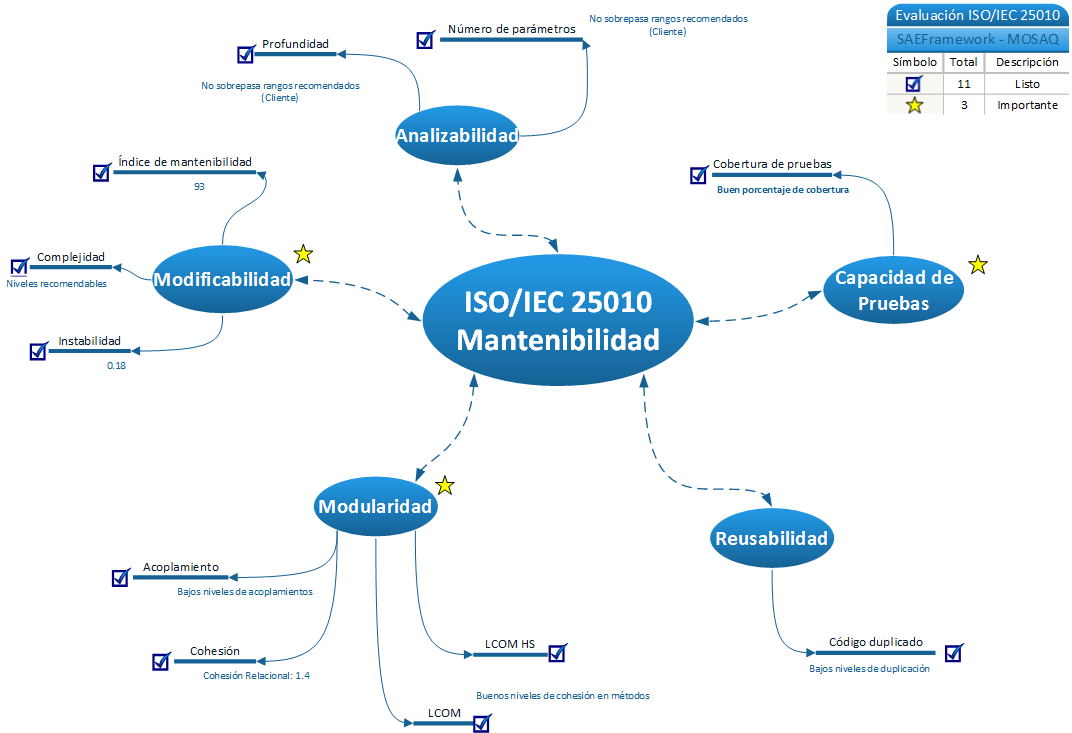
\includegraphics[width=1\textwidth]{img/diagrama.png}
%     \caption{Diagrama resumen de evaluación}
%     \label{fig:diagrama}
% \end{figure}

% MOSAQ: el modelo, descripciones cortas

\chapter{Conclusiones}
\label{chap:conclusiones}

\bibliographystyle{plain}
\bibliography{thesis}

\end{document}
